\documentclass[12pt,a4paper]{report}

% ========================================
% PACKAGES
% ========================================
\usepackage[utf8]{inputenc}
\usepackage[french]{babel}
\usepackage[T1]{fontenc}
\usepackage{geometry}
\geometry{a4paper, margin=2.5cm}
\usepackage{graphicx}
\usepackage{hyperref}
\usepackage{xcolor}
\usepackage{tikz}
\usepackage{pgf-umlcd}
\usepackage{listings}
\usepackage{fancyhdr}
\usepackage{titlesec}
\usepackage{tocloft}
\usepackage{booktabs}
\usepackage{longtable}
\usepackage{enumitem}
\usepackage{amsmath}
\usepackage{amssymb}
\usepackage{float}
\usepackage[ruled,vlined]{algorithm2e}
\usepackage{caption}
\usepackage{subcaption}
\usepackage{tabularx}

% Configuration des liens
\hypersetup{
    colorlinks=true,
    linkcolor=blue,
    filecolor=magenta,      
    urlcolor=cyan,
    citecolor=green,
    pdftitle={Rapport VoyageConnect},
    pdfauthor={},
    pdfsubject={Plateforme de réservation de voyages},
    pdfkeywords={Java EE, JSP, Servlets, JPA, Hibernate, MySQL}
}

% Configuration des en-têtes et pieds de page
\pagestyle{fancy}
\fancyhf{}
\fancyhead[L]{\leftmark}
\fancyhead[R]{VoyageConnect}
\fancyfoot[C]{\thepage}
\renewcommand{\headrulewidth}{0.4pt}
\renewcommand{\footrulewidth}{0.4pt}

% Configuration des titres de chapitres
\titleformat{\chapter}[display]
{\normalfont\huge\bfseries\color{blue!70!black}}
{\chaptertitlename\ \thechapter}{20pt}{\Huge}

% TikZ libraries pour UML
\usetikzlibrary{shapes,arrows,positioning,calc,fit,backgrounds}

% ========================================
% INFORMATIONS DU DOCUMENT
% ========================================
\title{
    \Huge \textbf{Développement d'une plateforme web\\de réservation de voyages}\\
    \vspace{1cm}
    \LARGE VoyageConnect\\
    \vspace{0.5cm}
    \large Projet de Développement Web Java EE
}

\author{
    \textbf{Nom et Prénom :} \textit{À COMPLÉTER}\\
    \vspace{0.3cm}
    \textbf{Établissement :} \textit{À COMPLÉTER}\\
    \textbf{Filière :} \textit{À COMPLÉTER}\\
    \vspace{0.3cm}
    \textbf{Encadrant pédagogique :} \textit{À COMPLÉTER}
}

\date{\textbf{Année universitaire :} 2024-2025\\
      \textbf{Date de soutenance :} \textit{À COMPLÉTER}}

\begin{document}

% ========================================
% PAGE DE GARDE
% ========================================
\begin{titlepage}
    \centering
    \vspace*{1cm}
    
    {\scshape\LARGE \textbf{NOM DE L'ÉTABLISSEMENT} \par}
    \vspace{0.5cm}
    {\scshape\Large \textbf{FILIÈRE / DÉPARTEMENT} \par}
    \vspace{2cm}
    
    {\huge\bfseries Développement d'une plateforme web de réservation de voyages\par}
    \vspace{0.5cm}
    {\LARGE\bfseries VoyageConnect\par}
    \vspace{2cm}
    
    {\Large\itshape Rapport de Projet\par}
    \vspace{1cm}
    
    \begin{minipage}{0.4\textwidth}
        \begin{flushleft} \large
            \textbf{Réalisé par :}\\
            \textit{NOM Prénom}\\
        \end{flushleft}
    \end{minipage}
    \hfill
    \begin{minipage}{0.4\textwidth}
        \begin{flushright} \large
            \textbf{Encadré par :}\\
            \textit{Nom Encadrant}\\
        \end{flushright}
    \end{minipage}
    
    \vfill
    
    {\large Année universitaire 2024-2025\par}
    {\large Date de soutenance : \textit{JJ/MM/AAAA}\par}
    
\end{titlepage}

% ========================================
% REMERCIEMENTS
% ========================================
\chapter*{Remerciements}
\addcontentsline{toc}{chapter}{Remerciements}

\vspace{1cm}

Au terme de ce projet, je tiens à exprimer ma profonde gratitude à toutes les personnes qui ont contribué, de près ou de loin, à la réalisation de cette plateforme web de réservation de voyages.

\vspace{0.5cm}

Mes sincères remerciements s'adressent en premier lieu à mon encadrant pédagogique, \textbf{\textit{Nom de l'encadrant}}, pour son accompagnement rigoureux, ses conseils avisés et sa disponibilité tout au long de ce projet. Ses orientations ont été déterminantes dans l'aboutissement de ce travail.

\vspace{0.5cm}

J'exprime également ma reconnaissance à l'ensemble du corps professoral de \textbf{\textit{Nom de l'établissement}} pour la qualité de l'enseignement dispensé, notamment en développement web, bases de données et architecture logicielle. Les connaissances acquises ont constitué le socle technique indispensable à la réalisation de ce projet.

\vspace{0.5cm}

Je remercie l'administration de l'établissement pour avoir mis à disposition les ressources matérielles et logicielles nécessaires au développement et aux tests de l'application.

\vspace{0.5cm}

Mes remerciements vont également à mes camarades de promotion pour les échanges constructifs et l'entraide qui ont enrichi mon apprentissage.

\vspace{0.5cm}

Enfin, je tiens à remercier ma famille et mes proches pour leur soutien constant et leurs encouragements durant toute la période de réalisation de ce projet.

\vspace{1cm}

\hfill \textit{Merci à tous.}

\clearpage

% ========================================
% RÉSUMÉ / ABSTRACT
% ========================================
\chapter*{Résumé}
\addcontentsline{toc}{chapter}{Résumé / Abstract}

\section*{Résumé}

Ce rapport présente le développement d'une plateforme web de réservation de voyages nommée \textbf{VoyageConnect}, réalisée dans le cadre d'un projet universitaire en développement web Java EE. L'objectif principal de ce projet est de concevoir et implémenter une solution informatique permettant de centraliser la recherche et la réservation de différents services touristiques : vols, hôtels et circuits organisés.

\vspace{0.3cm}

La méthodologie adoptée repose sur l'architecture Model-View-Controller (MVC) avec les technologies Java EE, notamment les Servlets pour la logique métier, JSP pour la couche présentation, JPA/Hibernate pour la persistance des données et MySQL comme système de gestion de base de données. Le serveur d'applications Apache Tomcat assure le déploiement de l'application.

\vspace{0.3cm}

Les principales fonctionnalités implémentées comprennent : un système d'authentification et de gestion des utilisateurs avec deux profils distincts (utilisateur et administrateur), un moteur de recherche multicritères pour les vols, hôtels et circuits, un système de réservation avec gestion transactionnelle atomique, un module de paiement simulé, et une interface d'administration pour la gestion du catalogue.

\vspace{0.3cm}

Les résultats obtenus démontrent la viabilité technique de la solution proposée. L'application permet de gérer efficacement l'ensemble du processus de réservation, de la recherche jusqu'à la confirmation du paiement, tout en garantissant l'intégrité des données grâce à la gestion des transactions JPA.

\vspace{0.3cm}

En conclusion, ce projet a permis d'acquérir une expérience pratique significative dans le développement d'applications web multi-couches en Java EE, la modélisation de bases de données relationnelles complexes et la mise en œuvre des bonnes pratiques de développement logiciel.

\vspace{0.5cm}

\noindent\textbf{Mots-clés :} Java EE, Servlet, JSP, JPA, Hibernate, MySQL, MVC, Réservation en ligne, Plateforme touristique, Apache Tomcat

\clearpage



% ========================================
% TABLE DES MATIÈRES
% ========================================
\tableofcontents
\clearpage

% Liste des figures
\listoffigures
\clearpage

% Liste des tableaux
\listoftables
\clearpage

% ========================================
% NOTE IMPORTANTE
% ========================================
% Pour compiler ce rapport dans Overleaf :
% 1. Créez un nouveau projet
% 2. Uploadez ce fichier en tant que main.tex
% 3. Compilez (cela peut prendre 1-2 minutes)
%
% ATTENTION : Les diagrammes UML avec stick figures sont remplacés par
% des cercles simples car l'option "stick figure" n'existe pas dans 
% pgf-umlcd standard. Vous pouvez les dessiner manuellement si besoin.
% ========================================

% Les fichiers suivants sont déjà intégrés dans ce document
% \input{01_introduction.tex}
% \input{02_chapitre1.tex}
% \input{03_chapitre2_partie1.tex}
% \input{04_chapitre2_partie2.tex}
% \input{05_chapitre3.tex}
% \input{06_conclusion.tex}



% ========================================
% INTRODUCTION
% ========================================
\chapter*{Introduction générale}
\addcontentsline{toc}{chapter}{Introduction générale}

\section*{Contexte général}

À l'ère du numérique, le secteur du tourisme connaît une transformation profonde avec la dématérialisation croissante des services de réservation. Les plateformes en ligne sont devenues incontournables pour les voyageurs souhaitant organiser leurs déplacements de manière autonome et efficace. Cette évolution technologique répond à un besoin grandissant de simplicité, de rapidité et de centralisation dans la planification des voyages.

\vspace{0.3cm}

Le marché de la réservation en ligne représente aujourd'hui un enjeu économique majeur, avec des acteurs internationaux tels que Booking.com, Expedia ou Airbnb qui dominent le secteur. Ces plateformes illustrent la pertinence d'une approche intégrée permettant de comparer et de réserver différents services touristiques au sein d'une interface unique.

\vspace{0.3cm}

C'est dans ce contexte que s'inscrit le projet \textbf{VoyageConnect}, une plateforme web de réservation de voyages développée avec les technologies Java EE. Ce projet vise à reproduire, à l'échelle académique, les fonctionnalités essentielles d'une agence de voyage en ligne, tout en mettant en œuvre les bonnes pratiques du développement web d'applications d'entreprise.

\section*{Problématique}

Actuellement, les voyageurs sont confrontés à plusieurs difficultés lorsqu'ils souhaitent organiser leurs déplacements :

\begin{itemize}
    \item \textbf{Fragmentation de l'information} : La nécessité de consulter plusieurs sites web différents pour comparer les offres de vols, d'hébergements et d'activités touristiques.
    
    \item \textbf{Manque de centralisation} : L'absence d'une plateforme unique permettant de gérer l'ensemble du processus de réservation, de la recherche au paiement.
    
    \item \textbf{Complexité du processus} : Les multiples étapes et interfaces différentes rendent l'expérience utilisateur peu intuitive et chronophage.
    
    \item \textbf{Absence de suivi} : La difficulté à centraliser et consulter l'historique de ses réservations lorsqu'elles sont effectuées sur différentes plateformes.
\end{itemize}

\vspace{0.3cm}

Face à ces constats, la question centrale de ce projet est la suivante : \textit{Comment concevoir et développer une plateforme web intégrée permettant de simplifier et de centraliser le processus de recherche et de réservation de services touristiques, tout en garantissant la fiabilité et la sécurité des transactions ?}

\section*{Objectifs du projet}

Le projet VoyageConnect poursuit plusieurs objectifs complémentaires :

\subsection*{Objectifs fonctionnels}

\begin{enumerate}
    \item \textbf{Développer un système de gestion des utilisateurs} comprenant l'inscription, l'authentification sécurisée et la gestion de profils (utilisateur standard et administrateur).
    
    \item \textbf{Implémenter un moteur de recherche multicritères} permettant de rechercher des vols, des hôtels et des circuits touristiques selon différents paramètres (destination, dates, prix, etc.).
    
    \item \textbf{Créer un système de réservation transactionnel} garantissant l'intégrité des données et la cohérence des réservations avec gestion atomique des paiements.
    
    \item \textbf{Concevoir une interface d'administration} permettant aux gestionnaires de maintenir le catalogue de services (ajout, modification, suppression de vols, hôtels et circuits).
    
    \item \textbf{Mettre en place un système de paiement simulé} reproduisant le flux d'une transaction réelle avec validation et confirmation.
\end{enumerate}

\subsection*{Objectifs techniques}

\begin{enumerate}
    \item Appliquer l'architecture Model-View-Controller (MVC) pour structurer l'application de manière modulaire et maintenable.
    
    \item Utiliser les technologies Java EE (Servlets, JSP) pour le développement de la couche web.
    
    \item Implémenter la persistance des données avec JPA/Hibernate et une base de données relationnelle MySQL.
    
    \item Garantir la gestion transactionnelle des opérations critiques (réservations, paiements).
    
    \item Développer une interface utilisateur responsive et intuitive utilisant Bootstrap.
    
    \item Assurer la validation des données côté serveur et côté client.
\end{enumerate}

\subsection*{Objectifs pédagogiques}

\begin{enumerate}
    \item Acquérir une maîtrise pratique du développement d'applications web Java EE.
    
    \item Appliquer les concepts de modélisation de bases de données relationnelles complexes.
    
    \item Comprendre et mettre en œuvre les principes de l'architecture multi-couches.
    
    \item Développer des compétences en gestion de projet et en documentation technique.
    
    \item Appréhender les enjeux de sécurité et d'intégrité des données dans les applications web.
\end{enumerate}

\section*{Structure du rapport}

Ce rapport est organisé en trois chapitres principaux :

\begin{itemize}
    \item \textbf{Chapitre 1 -- Problématique et contexte} : Présente l'état de l'art des technologies utilisées, les projets similaires existants et définit précisément la problématique ainsi que les objectifs du projet.
    
    \item \textbf{Chapitre 2 -- Méthodologie} : Détaille l'analyse des besoins, la conception de l'application (architecture, modélisation UML, structure de la base de données), les choix technologiques et la démarche de développement adoptée.
    
    \item \textbf{Chapitre 3 -- Réalisation du projet} : Décrit l'implémentation technique, présente les principales fonctionnalités développées, analyse les résultats obtenus et discute des problèmes rencontrés ainsi que des solutions apportées.
\end{itemize}

\vspace{0.5cm}

Le rapport se conclut par un bilan du projet, une synthèse des compétences acquises et une réflexion sur les perspectives d'évolution de la plateforme.

\clearpage



% ========================================
% CHAPITRE 1 : PROBLÉMATIQUE ET CONTEXTE
% ========================================
\chapter{Problématique et contexte}

\section{État de l'art et revue technologique}

Cette section présente les technologies et les concepts fondamentaux utilisés dans le développement de la plateforme VoyageConnect, ainsi qu'une analyse comparative des solutions existantes dans le domaine de la réservation de voyages en ligne.

\subsection{Technologies Java EE pour les applications web}

\subsubsection{Java Enterprise Edition (Java EE)}

Java Enterprise Edition est une plateforme de développement d'applications d'entreprise robustes, évolutives et sécurisées. Elle offre un ensemble de spécifications et d'APIs standardisées facilitant le développement d'applications distribuées multi-couches. Les principaux avantages de Java EE incluent :

\begin{itemize}
    \item \textbf{Portabilité} : Le code Java fonctionne sur n'importe quelle plateforme supportant la JVM.
    \item \textbf{Scalabilité} : Architecture conçue pour supporter la montée en charge.
    \item \textbf{Sécurité} : Mécanismes intégrés de gestion de l'authentification et des autorisations.
    \item \textbf{Gestion transactionnelle} : Support natif des transactions distribuées (JTA).
    \item \textbf{Écosystème mature} : Large communauté et nombreuses bibliothèques tierces.
\end{itemize}

\subsubsection{Servlets Java}

Les Servlets constituent la technologie de base pour le traitement des requêtes HTTP en Java. Un Servlet est une classe Java qui étend les capacités d'un serveur web en générant du contenu dynamique. Dans le contexte de VoyageConnect, les Servlets assurent :

\begin{itemize}
    \item Le routage des requêtes HTTP vers les traitements appropriés
    \item L'exécution de la logique métier
    \item La préparation des données pour la couche présentation
    \item La gestion des sessions utilisateurs
    \item Le contrôle d'accès et l'authentification
\end{itemize}

Le cycle de vie d'un Servlet comprend trois phases principales : initialisation (méthode \texttt{init()}), traitement des requêtes (méthodes \texttt{doGet()}, \texttt{doPost()}), et destruction (méthode \texttt{destroy()}).

\subsubsection{JavaServer Pages (JSP)}

JSP est une technologie permettant de créer des pages web dynamiques en embarquant du code Java dans du HTML. Les JSP sont automatiquement compilées en Servlets par le conteneur web. Les avantages des JSP incluent :

\begin{itemize}
    \item Séparation du code de présentation et de la logique métier
    \item Support de la bibliothèque JSTL (JSP Standard Tag Library) pour les opérations courantes
    \item Intégration aisée des Expression Language (EL) pour l'accès aux données
    \item Réutilisabilité via les directives include et les Custom Tags
\end{itemize}

Dans VoyageConnect, les JSP sont utilisées exclusivement pour la couche présentation, respectant ainsi le principe de séparation des préoccupations.

\subsection{Persistance des données avec JPA et Hibernate}

\subsubsection{Java Persistence API (JPA)}

JPA est une spécification Java définissant une interface de programmation pour la persistance objet-relationnelle (ORM). Elle permet de mapper des objets Java vers des tables de bases de données relationnelles, simplifiant ainsi considérablement les opérations CRUD (Create, Read, Update, Delete).

Les concepts clés de JPA comprennent :

\begin{itemize}
    \item \textbf{Entités} : Classes Java annotées représentant des tables de base de données
    \item \textbf{EntityManager} : Interface principale pour interagir avec le contexte de persistance
    \item \textbf{JPQL} : Langage de requêtes orienté objet similaire à SQL
    \item \textbf{Transactions} : Gestion de l'intégrité des données via les transactions JPA
    \item \textbf{Relations} : Mapping des associations entre entités (@OneToMany, @ManyToOne, @ManyToMany)
\end{itemize}

\subsubsection{Hibernate}

Hibernate est l'implémentation la plus populaire de la spécification JPA. Il fournit des fonctionnalités avancées telles que :

\begin{itemize}
    \item Gestion automatique du cache de premier et deuxième niveau
    \item Support du lazy loading pour optimiser les performances
    \item Génération automatique des schémas de base de données
    \item Support des requêtes HQL (Hibernate Query Language) et Criteria API
    \item Gestion sophistiquée des transactions et des verrous pessimistes/optimistes
\end{itemize}

Dans VoyageConnect, Hibernate assure la persistance de 9 entités principales (User, Flight, Hotel, Circuit, Reservation, Payment, Destination, Review, Promotion) avec leurs relations complexes.

\subsection{Architecture Model-View-Controller (MVC)}

L'architecture MVC est un patron de conception architectural qui sépare une application en trois composants principaux :

\begin{enumerate}
    \item \textbf{Modèle (Model)} : Représente les données de l'application et la logique métier. Dans VoyageConnect, le modèle comprend :
    \begin{itemize}
        \item Les entités JPA (User, Reservation, Flight, etc.)
        \item Les classes DAO (Data Access Object) pour l'accès aux données
        \item Les services métier (UserService, ReservationService, etc.)
    \end{itemize}
    
    \item \textbf{Vue (View)} : Responsable de la présentation des données à l'utilisateur. Elle inclut :
    \begin{itemize}
        \item Les pages JSP pour l'affichage
        \item Les fichiers CSS pour le style
        \item Les scripts JavaScript pour l'interactivité côté client
    \end{itemize}
    
    \item \textbf{Contrôleur (Controller)} : Gère les interactions utilisateur et coordonne le modèle et la vue :
    \begin{itemize}
        \item Les Servlets Java traitant les requêtes HTTP
        \item Les filtres pour l'authentification et l'autorisation
        \item La logique de routage et de navigation
    \end{itemize}
\end{enumerate}

Les avantages de l'architecture MVC incluent une meilleure maintenabilité, une réutilisabilité accrue du code, une facilitation des tests unitaires et une séparation claire des responsabilités.

\subsection{Système de gestion de base de données MySQL}

MySQL est un système de gestion de base de données relationnelle open source largement utilisé dans les applications web. Ses caractéristiques principales sont :

\begin{itemize}
    \item \textbf{Performance} : Optimisé pour les opérations de lecture rapides
    \item \textbf{Fiabilité} : Support complet des transactions ACID via le moteur InnoDB
    \item \textbf{Scalabilité} : Capacité à gérer de grandes quantités de données
    \item \textbf{Sécurité} : Système robuste de gestion des utilisateurs et des privilèges
    \item \textbf{Compatibilité} : Excellente intégration avec Java via le driver JDBC
\end{itemize}

Pour VoyageConnect, MySQL stocke l'ensemble des données de l'application dans 9 tables principales avec des relations complexes (clés étrangères, contraintes d'intégrité référentielle).

\subsection{Serveur d'applications Apache Tomcat}

Apache Tomcat est un conteneur de servlets et de JSP open source développé par la fondation Apache. Il implémente les spécifications Java Servlet et JavaServer Pages. Tomcat est choisi pour ce projet en raison de :

\begin{itemize}
    \item Sa légèreté et sa simplicité de configuration
    \item Sa conformité aux spécifications Java EE
    \item Sa robustesse et sa stabilité éprouvée
    \item Son large support communautaire
    \item Sa gratuité et sa nature open source
\end{itemize}

\subsection{Frameworks et bibliothèques complémentaires}

\subsubsection{Bootstrap}

Bootstrap est un framework CSS responsive permettant de créer rapidement des interfaces web modernes et adaptatives. Il offre :

\begin{itemize}
    \item Un système de grille flexible pour le responsive design
    \item Des composants UI préconçus (boutons, formulaires, modales, etc.)
    \item Une cohérence visuelle sur tous les navigateurs
    \item Une documentation exhaustive et une grande communauté
\end{itemize}

\subsubsection{JSTL (JSP Standard Tag Library)}

JSTL fournit un ensemble de balises personnalisées pour les opérations courantes dans les JSP :

\begin{itemize}
    \item Balises de contrôle de flux (\texttt{<c:if>}, \texttt{<c:forEach>})
    \item Balises de formatage (\texttt{<fmt:formatDate>}, \texttt{<fmt:formatNumber>})
    \item Balises pour les opérations SQL et XML
\end{itemize}

\subsection{Méthodologies de développement}

\subsubsection{Développement itératif et incrémental}

Le projet VoyageConnect a été développé selon une approche itérative, permettant de livrer des fonctionnalités progressivement testées et validées. Cette méthodologie présente plusieurs avantages :

\begin{itemize}
    \item Détection précoce des problèmes et des erreurs de conception
    \item Adaptation facilitée aux changements de requirements
    \item Motivation accrue grâce à des résultats tangibles réguliers
    \item Réduction des risques projet
\end{itemize}

\subsubsection{Gestion de versions avec Git}

Git est utilisé pour le contrôle de version du code source, offrant :

\begin{itemize}
    \item Un historique complet des modifications
    \item La possibilité de travailler sur plusieurs fonctionnalités en parallèle (branches)
    \item La sauvegarde sécurisée du code sur des dépôts distants (GitHub)
    \item La collaboration facilitée entre développeurs
\end{itemize}

\subsection{Analyse comparative : projets similaires}

\subsubsection{Booking.com}

Booking.com est une plateforme leader mondiale dans la réservation d'hébergements. Ses points forts incluent :

\begin{itemize}
    \item Interface utilisateur intuitive et multilingue
    \item Système de recherche avancé avec filtres multiples
    \item Système d'avis clients fiable
    \item Gestion complète du processus de réservation
    \item Application mobile performante
\end{itemize}

\textbf{Enseignements pour VoyageConnect} : Importance d'un moteur de recherche performant, nécessité d'une interface claire et d'un système de confirmation de réservation robuste.

\subsubsection{Expedia}

Expedia offre une approche intégrée combinant vols, hôtels et locations de voiture. Ses caractéristiques principales :

\begin{itemize}
    \item Packages combinés (vol + hôtel) avec réductions
    \item Programme de fidélité avec points cumulables
    \item Assistance client 24/7
    \item Gestion centralisée des réservations
\end{itemize}

\textbf{Enseignements pour VoyageConnect} : Pertinence d'une approche multi-services, importance de la centralisation des réservations dans un tableau de bord utilisateur.

\subsubsection{Airbnb}

Airbnb a révolutionné le marché de l'hébergement touristique avec son modèle de plateforme communautaire :

\begin{itemize}
    \item Interface moderne et design soigné
    \item Système de confiance basé sur les avis
    \item Profils détaillés des hôtes et des logements
    \item Communication intégrée entre voyageurs et hôtes
\end{itemize}

\textbf{Enseignements pour VoyageConnect} : Importance du design UX/UI, valeur ajoutée des systèmes d'avis et de notation.

\subsection{Synthèse de l'état de l'art}

L'analyse des technologies existantes et des plateformes concurrentes révèle plusieurs exigences fondamentales pour le développement de VoyageConnect :

\begin{enumerate}
    \item Adoption d'une architecture robuste et évolutive (MVC + Java EE)
    \item Utilisation d'un ORM performant pour la gestion des données (JPA/Hibernate)
    \item Conception d'une interface utilisateur responsive et intuitive
    \item Mise en place d'un système de gestion transactionnelle fiable
    \item Implémentation de mécanismes de sécurité appropriés
\end{enumerate}

\section{Problématique et objectifs du projet}

\subsection{Définition de la problématique}

Le secteur du tourisme en ligne fait face à plusieurs défis majeurs qui constituent la problématique centrale de ce projet :

\subsubsection{Fragmentation des services}

Les voyageurs doivent naviguer entre de multiples plateformes spécialisées pour organiser un voyage complet. Cette fragmentation entraîne :

\begin{itemize}
    \item Une perte de temps considérable dans la comparaison des offres
    \item Une difficulté à obtenir une vue d'ensemble cohérente du voyage
    \item Des risques d'incohérence entre les différentes réservations (dates, destinations)
    \item Une multiplication des comptes utilisateurs et des données personnelles dispersées
\end{itemize}

\subsubsection{Complexité du processus de réservation}

Le parcours utilisateur pour effectuer une réservation est souvent complexe et peu ergonomique :

\begin{itemize}
    \item Formulaires longs et répétitifs
    \item Processus de paiement morcelé
    \item Manque de feedback en temps réel sur la disponibilité
    \item Absence de confirmation immédiate
\end{itemize}

\subsubsection{Gestion décentralisée des réservations}

L'absence d'un point central de gestion pose plusieurs problèmes :

\begin{itemize}
    \item Difficulté à retrouver les confirmations de réservation
    \item Impossibilité de modifier ou annuler facilement
    \item Absence d'historique complet des voyages
    \item Notifications dispersées sur plusieurs canaux
\end{itemize}

\subsubsection{Fiabilité et sécurité des transactions}

Les utilisateurs expriment des préoccupations légitimes concernant :

\begin{itemize}
    \item La sécurité de leurs données de paiement
    \item La garantie de la réservation effective après paiement
    \item La protection contre les doubles réservations
    \item La confidentialité de leurs données personnelles
\end{itemize}

\subsection{Formulation de la problématique}

Au regard de ces constats, la problématique du projet VoyageConnect peut être formulée ainsi :

\begin{quote}
\textit{Comment concevoir et développer une plateforme web intégrée de réservation de services touristiques (vols, hôtels, circuits) qui centralise l'ensemble du processus depuis la recherche jusqu'à la confirmation de paiement, tout en garantissant la fiabilité des transactions, la sécurité des données et une expérience utilisateur optimale, en utilisant les technologies Java EE et une architecture MVC ?}
\end{quote}

\subsection{Objectifs du projet}

Pour répondre à cette problématique, le projet VoyageConnect poursuit les objectifs suivants :

\subsubsection{Objectif général}

Développer une plateforme web complète et fonctionnelle de réservation de voyages permettant aux utilisateurs de rechercher, comparer et réserver des vols, des hôtels et des circuits touristiques via une interface unique, sécurisée et intuitive.

\subsubsection{Objectifs fonctionnels}

\begin{enumerate}
    \item \textbf{Gestion des utilisateurs}
    \begin{itemize}
        \item Système d'inscription avec validation des données
        \item Authentification sécurisée (hashage des mots de passe)
        \item Gestion de profils (utilisateur standard, administrateur)
        \item Maintien de sessions utilisateur
    \end{itemize}
    
    \item \textbf{Recherche de services touristiques}
    \begin{itemize}
        \item Moteur de recherche multicritères pour les vols (destination, dates, classe)
        \item Recherche d'hôtels (destination, étoiles, équipements)
        \item Recherche de circuits (destination, durée, prix)
        \item Affichage des résultats avec tri et filtrage
    \end{itemize}
    
    \item \textbf{Système de réservation}
    \begin{itemize}
        \item Création de réservations pour vols, hôtels et circuits
        \item Vérification en temps réel de la disponibilité
        \item Calcul automatique du montant total
        \item Gestion transactionnelle atomique (réservation + paiement indissociables)
        \item Confirmation immédiate avec numéro de réservation unique
    \end{itemize}
    
    \item \textbf{Gestion des réservations}
    \begin{itemize}
        \item Tableau de bord utilisateur affichant toutes les réservations
        \item Consultation des détails de chaque réservation
        \item Possibilité d'annulation (avec gestion du statut)
        \item Historique complet des réservations
    \end{itemize}
    
    \item \textbf{Module de paiement}
    \begin{itemize}
        \item Simulation de paiement par carte bancaire, PayPal ou virement
        \item Validation des informations de paiement
        \item Enregistrement sécurisé des transactions
        \item Confirmation de paiement
    \end{itemize}
    
    \item \textbf{Interface d'administration}
    \begin{itemize}
        \item Gestion du catalogue de vols (ajout, modification, suppression)
        \item Gestion des hôtels et de leurs équipements
        \item Gestion des circuits touristiques
        \item Consultation de toutes les réservations
        \item Statistiques d'utilisation de la plateforme
    \end{itemize}
\end{enumerate}

\subsubsection{Objectifs techniques}

\begin{enumerate}
    \item \textbf{Architecture}
    \begin{itemize}
        \item Implémentation stricte du pattern MVC
        \item Séparation claire des couches (présentation, métier, données)
        \item Modularité et réutilisabilité du code
    \end{itemize}
    
    \item \textbf{Développement web}
    \begin{itemize}
        \item Utilisation de Servlets Java pour les contrôleurs
        \item Pages JSP avec JSTL pour la présentation
        \item Filtres pour l'authentification et les autorisations
        \item Gestion appropriée des sessions HTTP
    \end{itemize}
    
    \item \textbf{Persistance}
    \begin{itemize}
        \item Modélisation complète des entités avec JPA
        \item Mapping des relations entre entités (OneToMany, ManyToOne)
        \item Implémentation du pattern DAO
        \item Gestion des transactions avec EntityManager
    \end{itemize}
    
    \item \textbf{Base de données}
    \begin{itemize}
        \item Conception d'un schéma relationnel normalisé
        \item Respect des contraintes d'intégrité référentielle
        \item Optimisation des requêtes
        \item Indexation appropriée des tables
    \end{itemize}
    
    \item \textbf{Sécurité}
    \begin{itemize}
        \item Validation des données côté serveur
        \item Protection contre les injections SQL (requêtes paramétrées)
        \item Hashage des mots de passe (algorithme BCrypt)
        \item Contrôle d'accès basé sur les rôles
    \end{itemize}
    
    \item \textbf{Interface utilisateur}
    \begin{itemize}
        \item Design responsive (Bootstrap)
        \item Navigation intuitive
        \item Feedback utilisateur approprié (messages d'erreur, confirmations)
        \item Validation côté client (JavaScript)
    \end{itemize}
\end{enumerate}

\subsubsection{Objectifs pédagogiques}

Ce projet vise également à développer des compétences pratiques essentielles :

\begin{enumerate}
    \item Maîtrise du développement d'applications web Java EE multi-couches
    \item Compétences en modélisation et conception de bases de données relationnelles
    \item Capacité à implémenter une architecture logicielle robuste et maintenable
    \item Compréhension des enjeux de sécurité dans les applications web
    \item Aptitude à gérer un projet de développement de A à Z
    \item Compétences en documentation technique et rédaction de rapports
\end{enumerate}

\subsection{Périmètre du projet}

\subsubsection{Fonctionnalités incluses}

\begin{itemize}
    \item Gestion complète des utilisateurs (inscription, connexion, profils)
    \item Recherche et réservation de vols, hôtels et circuits
    \item Système de paiement simulé (sans intégration réelle de passerelle de paiement)
    \item Tableau de bord utilisateur
    \item Interface d'administration complète
    \item Gestion transactionnelle des réservations
\end{itemize}

\subsubsection{Fonctionnalités exclues (perspectives d'évolution)}

\begin{itemize}
    \item Intégration de passerelles de paiement réelles
    \item Application mobile native
    \item Système de recommandations basé sur l'IA
    \item Notifications email automatiques
    \item Système de fidélité et de points
    \item Comparaison de prix avec des sites externes
    \item Génération de factures PDF
    \item Système de messagerie entre utilisateurs et administrateurs
\end{itemize}

\subsection{Contraintes du projet}

\subsubsection{Contraintes techniques}

\begin{itemize}
    \item Utilisation obligatoire des technologies Java EE (Servlets, JSP)
    \item Implémentation avec JPA/Hibernate pour la persistance
    \item Déploiement sur Apache Tomcat
    \item Base de données relationnelle MySQL
    \item Architecture MVC stricte
\end{itemize}

\subsubsection{Contraintes temporelles}

\begin{itemize}
    \item Développement dans le cadre d'un semestre académique
    \item Livraison d'une version fonctionnelle pour la soutenance
    \item Documentation complète du projet
\end{itemize}

\subsubsection{Contraintes de ressources}

\begin{itemize}
    \item Projet individuel (pas de travail en équipe)
    \item Ressources matérielles limitées (environnement de développement local)
    \item Pas de budget pour des services payants (API, hébergement cloud)
\end{itemize}

\subsection{Indicateurs de succès}

Le succès du projet sera évalué selon les critères suivants :

\begin{enumerate}
    \item \textbf{Fonctionnalité} : Toutes les fonctionnalités principales sont opérationnelles
    \item \textbf{Fiabilité} : Gestion correcte des transactions sans perte de données
    \item \textbf{Utilisabilité} : Interface intuitive et navigation fluide
    \item \textbf{Performance} : Temps de réponse acceptables pour les opérations courantes
    \item \textbf{Sécurité} : Implémentation des bonnes pratiques de sécurité web
    \item \textbf{Qualité du code} : Code structuré, commenté et maintenable
    \item \textbf{Documentation} : Rapport complet et documentation technique claire
\end{enumerate}

\clearpage



% ========================================
% CHAPITRE 2 : MÉTHODOLOGIE
% ========================================
\chapter{Méthodologie}

\section{Analyse des besoins}

L'analyse des besoins constitue la première étape fondamentale du développement de la plateforme VoyageConnect. Elle permet d'identifier précisément les fonctionnalités attendues et les contraintes du système.

\subsection{Identification des acteurs}

Le système VoyageConnect interagit avec deux types d'acteurs principaux :

\begin{table}[H]
\centering
\caption{Acteurs du système VoyageConnect}
\label{tab:acteurs}
\begin{tabular}{|l|p{10cm}|}
\hline
\textbf{Acteur} & \textbf{Description et responsabilités} \\
\hline
\textbf{Utilisateur} (USER) & Client de la plateforme pouvant s'inscrire, se connecter, rechercher des services touristiques (vols, hôtels, circuits), effectuer des réservations, procéder aux paiements et consulter l'historique de ses réservations. \\
\hline
\textbf{Administrateur} (ADMIN) & Gestionnaire de la plateforme ayant accès à toutes les fonctionnalités utilisateur plus les droits de gestion du catalogue (ajout, modification, suppression de vols, hôtels, circuits), consultation de toutes les réservations et accès aux statistiques de la plateforme. \\
\hline
\end{tabular}
\end{table}

\subsection{Besoins fonctionnels}

Les besoins fonctionnels décrivent les fonctionnalités que le système doit offrir aux utilisateurs.

\subsubsection{BF1 : Gestion des utilisateurs}

\begin{itemize}
    \item \textbf{BF1.1} : Un visiteur doit pouvoir s'inscrire en fournissant nom, prénom, email, mot de passe, téléphone et adresse.
    \item \textbf{BF1.2} : Le système doit valider l'unicité de l'adresse email lors de l'inscription.
    \item \textbf{BF1.3} : Les mots de passe doivent être hashés avant stockage en base de données.
    \item \textbf{BF1.4} : Un utilisateur inscrit doit pouvoir se connecter avec son email et mot de passe.
    \item \textbf{BF1.5} : Un utilisateur connecté doit pouvoir modifier son profil (nom, téléphone, adresse).
    \item \textbf{BF1.6} : Un utilisateur doit pouvoir se déconnecter, invalidant ainsi sa session.
\end{itemize}

\subsubsection{BF2 : Recherche de services touristiques}

\begin{itemize}
    \item \textbf{BF2.1} : Le système doit permettre la recherche de vols selon les critères : destination, date de départ, classe (Économique, Affaires, Première).
    \item \textbf{BF2.2} : Le système doit permettre la recherche d'hôtels selon les critères : destination, nombre d'étoiles, équipements disponibles.
    \item \textbf{BF2.3} : Le système doit permettre la recherche de circuits selon les critères : destination, durée, fourchette de prix.
    \item \textbf{BF2.4} : Les résultats de recherche doivent afficher toutes les informations pertinentes (prix, disponibilité, caractéristiques).
    \item \textbf{BF2.5} : Les utilisateurs non connectés doivent pouvoir effectuer des recherches.
\end{itemize}

\subsubsection{BF3 : Réservation de services}

\begin{itemize}
    \item \textbf{BF3.1} : Seuls les utilisateurs authentifiés peuvent effectuer des réservations.
    \item \textbf{BF3.2} : Lors d'une réservation de vol, le système doit vérifier la disponibilité des places.
    \item \textbf{BF3.3} : Lors d'une réservation d'hôtel, le système doit vérifier les disponibilités pour les dates spécifiées.
    \item \textbf{BF3.4} : Le système doit calculer automatiquement le montant total en fonction du nombre de personnes et du prix unitaire.
    \item \textbf{BF3.5} : Chaque réservation doit recevoir un numéro unique de confirmation.
    \item \textbf{BF3.6} : La création d'une réservation et le paiement associé doivent constituer une transaction atomique.
    \item \textbf{BF3.7} : En cas d'échec du paiement, la réservation doit être annulée automatiquement (rollback).
\end{itemize}

\subsubsection{BF4 : Gestion des réservations}

\begin{itemize}
    \item \textbf{BF4.1} : Un utilisateur doit pouvoir consulter la liste complète de ses réservations.
    \item \textbf{BF4.2} : Un utilisateur doit pouvoir consulter les détails d'une réservation spécifique.
    \item \textbf{BF4.3} : Un utilisateur doit pouvoir annuler une réservation en statut « En attente » ou « Confirmée ».
    \item \textbf{BF4.4} : Le système doit mettre à jour le statut de la réservation lors d'une annulation.
    \item \textbf{BF4.5} : Le tableau de bord utilisateur doit afficher un résumé des réservations avec leur statut.
\end{itemize}

\subsubsection{BF5 : Gestion des paiements}

\begin{itemize}
    \item \textbf{BF5.1} : Le système doit proposer trois méthodes de paiement : Carte bancaire, PayPal, Virement bancaire.
    \item \textbf{BF5.2} : Le système doit valider les informations de paiement fournies.
    \item \textbf{BF5.3} : Un paiement doit être lié de manière unique à une réservation.
    \item \textbf{BF5.4} : Le système doit enregistrer la date et l'heure de chaque transaction.
    \item \textbf{BF5.5} : Chaque paiement doit avoir un numéro de transaction unique.
\end{itemize}

\subsubsection{BF6 : Administration}

\begin{itemize}
    \item \textbf{BF6.1} : Un administrateur doit pouvoir ajouter, modifier et supprimer des vols.
    \item \textbf{BF6.2} : Un administrateur doit pouvoir ajouter, modifier et supprimer des hôtels.
    \item \textbf{BF6.3} : Un administrateur doit pouvoir ajouter, modifier et supprimer des circuits.
    \item \textbf{BF6.4} : Un administrateur doit pouvoir consulter toutes les réservations de tous les utilisateurs.
    \item \textbf{BF6.5} : Un administrateur doit avoir accès à des statistiques (nombre de réservations, chiffre d'affaires).
\end{itemize}

\subsection{Besoins non fonctionnels}

Les besoins non fonctionnels définissent les critères de qualité et les contraintes techniques du système.

\subsubsection{BNF1 : Performance}

\begin{itemize}
    \item Le temps de réponse pour une page d'affichage ne doit pas excéder 2 secondes.
    \item Le temps de réponse pour une recherche ne doit pas excéder 3 secondes.
    \item Le système doit pouvoir gérer au moins 100 utilisateurs simultanés.
\end{itemize}

\subsubsection{BNF2 : Sécurité}

\begin{itemize}
    \item Tous les mots de passe doivent être hashés avec un algorithme sécurisé (BCrypt).
    \item Les sessions utilisateur doivent expirer après 30 minutes d'inactivité.
    \item Le système doit être protégé contre les injections SQL.
    \item Les formulaires doivent être protégés contre les attaques XSS et CSRF.
\end{itemize}

\subsubsection{BNF3 : Fiabilité}

\begin{itemize}
    \item Le système doit garantir l'intégrité des transactions (ACID).
    \item Aucune réservation ne doit être perdue en cas d'erreur système.
    \item Le système doit éviter les doublons de réservations.
\end{itemize}

\subsubsection{BNF4 : Utilisabilité}

\begin{itemize}
    \item L'interface doit être responsive et s'adapter aux écrans mobiles, tablettes et desktop.
    \item Les messages d'erreur doivent être clairs et en français.
    \item La navigation doit être intuitive sans formation préalable.
\end{itemize}

\subsubsection{BNF5 : Maintenabilité}

\begin{itemize}
    \item Le code doit respecter les conventions de nommage Java.
    \item Le code doit être commenté et documenté.
    \item L'architecture MVC doit être strictement respectée.
    \item Les couches de l'application doivent être découplées.
\end{itemize}

\subsubsection{BNF6 : Portabilité}

\begin{itemize}
    \item L'application doit fonctionner sur tout système supportant Java 11+.
    \item L'application doit être compatible avec les navigateurs modernes (Chrome, Firefox, Edge, Safari).
\end{itemize}

\section{Conception du système}

La phase de conception traduit les besoins identifiés en modèles et schémas techniques guidant le développement.

\subsection{Architecture générale : Modèle MVC}

L'architecture de VoyageConnect repose sur le patron Model-View-Controller (MVC), garantissant une séparation claire des responsabilités et facilitant la maintenance et l'évolutivité du système.

\begin{figure}[H]
\centering
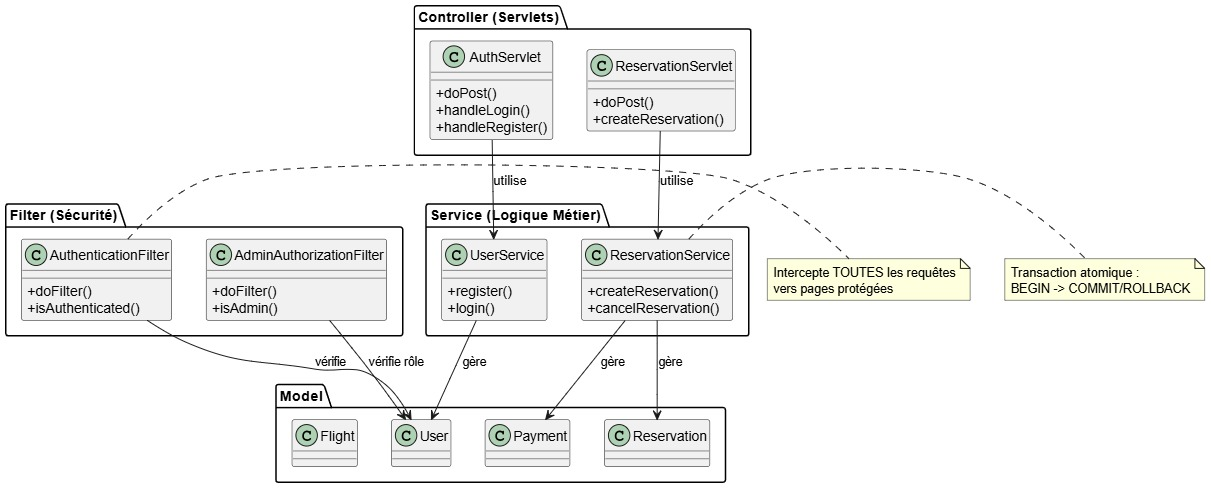
\includegraphics[width=0.9\textwidth]{diagrams/architectureMVC.jpeg}
\caption{Architecture MVC de VoyageConnect}
\label{fig:mvc}
\end{figure}

\subsubsection{Couche Modèle (Model)}

La couche modèle encapsule la logique métier et l'accès aux données. Elle comprend :

\begin{itemize}
    \item \textbf{Entités JPA} : 9 classes représentant les objets métier (User, Flight, Hotel, Circuit, Reservation, Payment, Destination, Review, Promotion)
    \item \textbf{DAOs (Data Access Objects)} : 10 classes assurant les opérations CRUD (Create, Read, Update, Delete)
    \item \textbf{Services métier} : 5 classes encapsulant la logique applicative (UserService, ReservationService, SearchService, etc.)
    \item \textbf{Classes utilitaires} : Gestion JPA, validation, hachage de mots de passe, envoi d'emails
\end{itemize}

\subsubsection{Couche Vue (View)}

La couche vue gère l'interface utilisateur et la présentation des données :

\begin{itemize}
    \item \textbf{Pages JSP} : 25+ pages organisées par fonctionnalité (/views/user/, /views/admin/, /views/reservation/, etc.)
    \item \textbf{Fragments réutilisables} : navbar.jsp, footer.jsp pour éviter la duplication de code
    \item \textbf{CSS} : Styles personnalisés combinés à Bootstrap pour le responsive design
    \item \textbf{JavaScript} : Validation côté client, interactivité dynamique
\end{itemize}

\subsubsection{Couche Contrôleur (Controller)}

La couche contrôleur orchestre les interactions entre le modèle et la vue :

\begin{itemize}
    \item \textbf{Servlets} : 12 servlets traitant les requêtes HTTP (AuthServlet, ReservationServlet, SearchServlet, etc.)
    \item \textbf{Filtres} : AuthenticationFilter, AdminAuthorizationFilter pour la sécurité
    \item \textbf{Gestion de sessions} : Maintien de l'état utilisateur connecté
\end{itemize}

\subsection{Modélisation UML}

La modélisation UML permet de représenter visuellement la structure et le comportement du système VoyageConnect. Nous présentons ici les trois diagrammes principaux : cas d'utilisation, classes et séquence.

\clearpage

\subsubsection{Diagramme de cas d'utilisation}

Le diagramme de cas d'utilisation illustre les interactions entre les acteurs (Visiteur, Utilisateur et Administrateur) et le système VoyageConnect.

\begin{figure}[H]
\centering
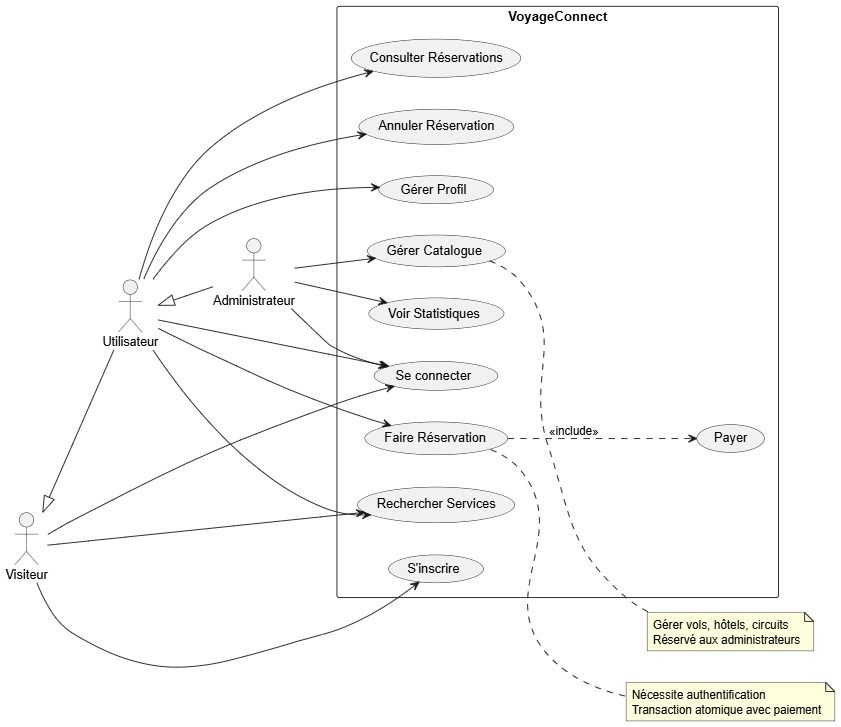
\includegraphics[width=0.95\textwidth]{diagrams/diagrammeDeCasDutilisation.jpeg}
\caption{Diagramme de cas d'utilisation de VoyageConnect}
\label{fig:usecase}
\end{figure}

\textbf{Description des cas d'utilisation principaux :}

\begin{itemize}
    \item \textbf{S'inscrire} : Permet à un visiteur de créer un compte utilisateur.
    \item \textbf{Se connecter} : Authentification d'un utilisateur existant.
    \item \textbf{Rechercher services} : Recherche multicritères de vols, hôtels ou circuits.
    \item \textbf{Réserver service} : Création d'une réservation (inclut obligatoirement le paiement).
    \item \textbf{Consulter réservations} : Affichage de l'historique des réservations.
    \item \textbf{Annuler réservation} : Annulation d'une réservation existante.
    \item \textbf{Gérer vols/hôtels/circuits} : Administration du catalogue (CRUD).
\end{itemize}

\clearpage

\subsubsection{Diagramme de classes}

Le diagramme de classes représente la structure statique du système, incluant les entités principales, leurs attributs et leurs relations.

\begin{figure}[H]
\centering
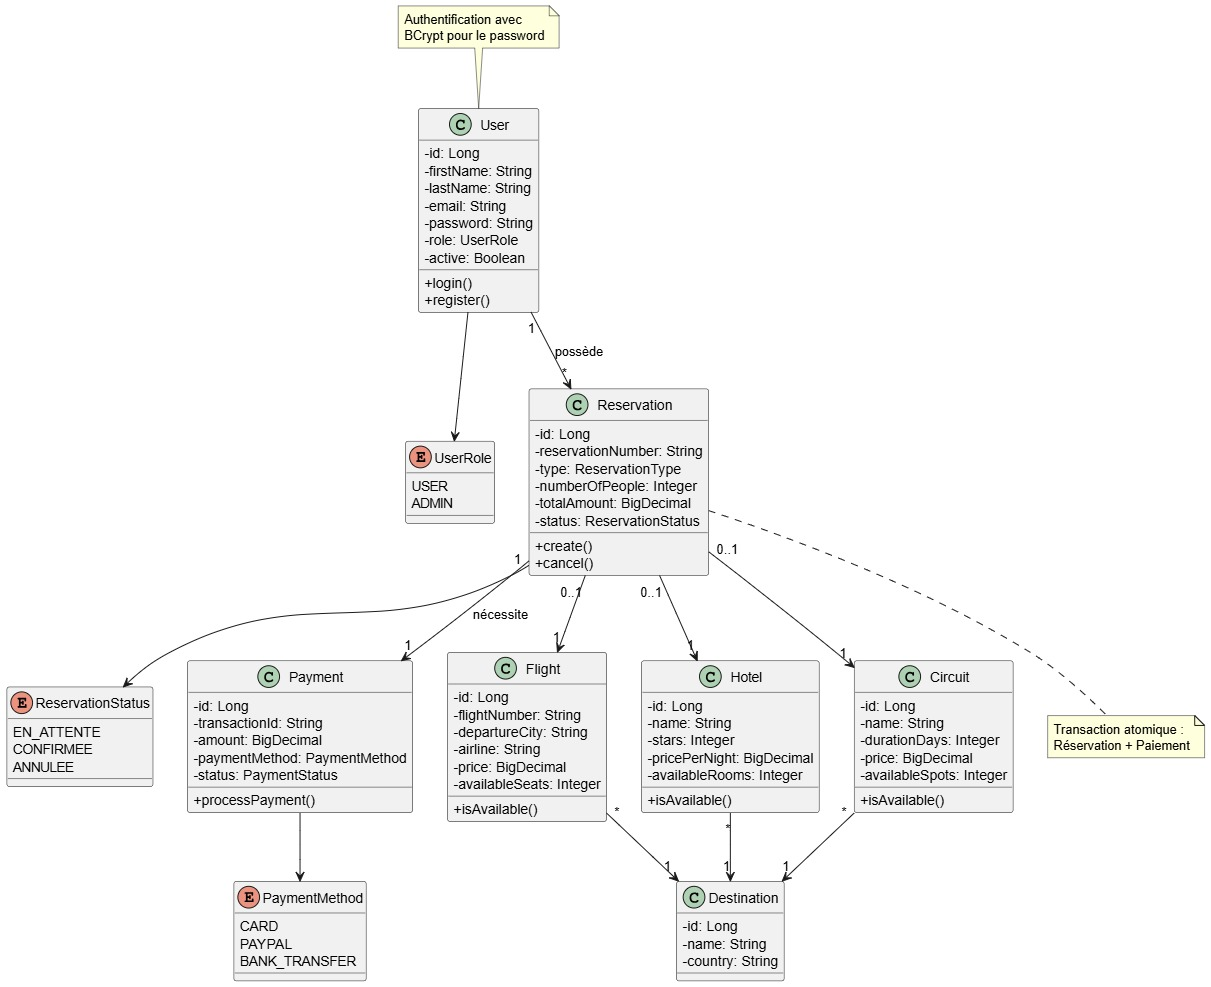
\includegraphics[width=1.0\textwidth]{diagrams/diagrammeDEClasse.jpeg}
\caption{Diagramme de classes simplifié de VoyageConnect}
\label{fig:classes}
\end{figure}

\textbf{Description des principales classes :}

\begin{itemize}
    \item \textbf{User} : Représente un utilisateur du système (client ou administrateur). Contient les informations personnelles et d'authentification.
    
    \item \textbf{Reservation} : Entité centrale gérant les réservations de vols, hôtels ou circuits. Liée obligatoirement à un paiement.
    
    \item \textbf{Flight} : Représente un vol avec ses caractéristiques (numéro, dates, prix, places disponibles).
    
    \item \textbf{Hotel} : Représente un hôtel avec ses équipements et tarifs.
    
    \item \textbf{Circuit} : Représente un circuit touristique organisé.
    
    \item \textbf{Payment} : Gère les transactions de paiement liées aux réservations.
    
    \item \textbf{Destination} : Représente une destination géographique (ville/pays).
    
    \item \textbf{Review} : Avis et évaluations laissés par les utilisateurs sur les services.
\end{itemize}

\textbf{Principaux cardinalités et relations :}

\begin{itemize}
    \item Un \texttt{User} peut avoir plusieurs \texttt{Reservation} (1..*)
    \item Une \texttt{Reservation} a exactement un \texttt{Payment} (1..1)
    \item Une \texttt{Reservation} est liée à un seul service : \texttt{Flight} OU \texttt{Hotel} OU \texttt{Circuit} (0..1)
    \item Tous les services (\texttt{Flight}, \texttt{Hotel}, \texttt{Circuit}) sont liés à une \texttt{Destination} (*.1)
    \item Un \texttt{User} peut laisser plusieurs \texttt{Review} (1..*)
\end{itemize}

\clearpage

\subsubsection{Diagrammes de séquence}

Les diagrammes de séquence illustrent les interactions entre les objets du système au fil du temps pour accomplir des fonctionnalités spécifiques. Nous présentons trois scénarios principaux.

\textbf{Diagramme de séquence 1 : Inscription d'un nouvel utilisateur}

\begin{figure}[H]
\centering
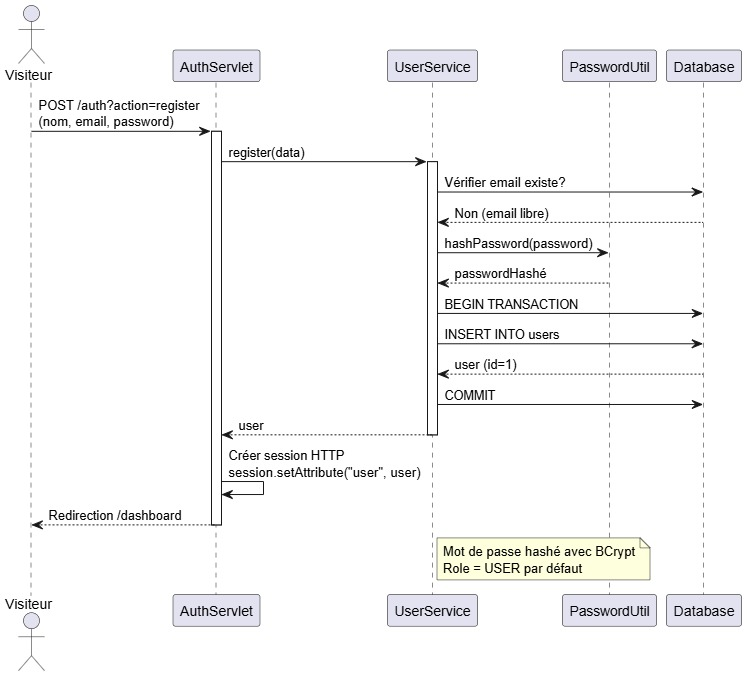
\includegraphics[width=0.95\textwidth]{diagrams/diagrammeSequenceInscription.jpeg}
\caption{Diagramme de séquence : Inscription}
\label{fig:seq-register}
\end{figure}

\textbf{Description du scénario :}

\begin{enumerate}
    \item L'utilisateur saisit son email et mot de passe dans le formulaire de connexion.
    \item Le formulaire JSP soumet une requête POST vers AuthServlet.
    \item AuthServlet appelle UserService pour authentifier l'utilisateur.
    \item UserService utilise UserDAO pour rechercher l'utilisateur par email.
    \item UserDAO exécute une requête SQL SELECT sur la base de données.
    \item La base retourne les données de l'utilisateur.
    \item UserDAO construit un objet User et le retourne au Service.
    \item UserService vérifie la correspondance entre le mot de passe saisi et le hash stocké.
    \item Si authentification réussie, UserService retourne l'objet User au Servlet.
    \item AuthServlet crée une session HTTP et y stocke l'utilisateur.
    \item Redirection vers le tableau de bord utilisateur.
    \item Affichage de la page dashboard.jsp.
\end{enumerate}

\clearpage

\textbf{Diagramme de séquence 2 : Connexion (Authentification)}

\begin{figure}[H]
\centering
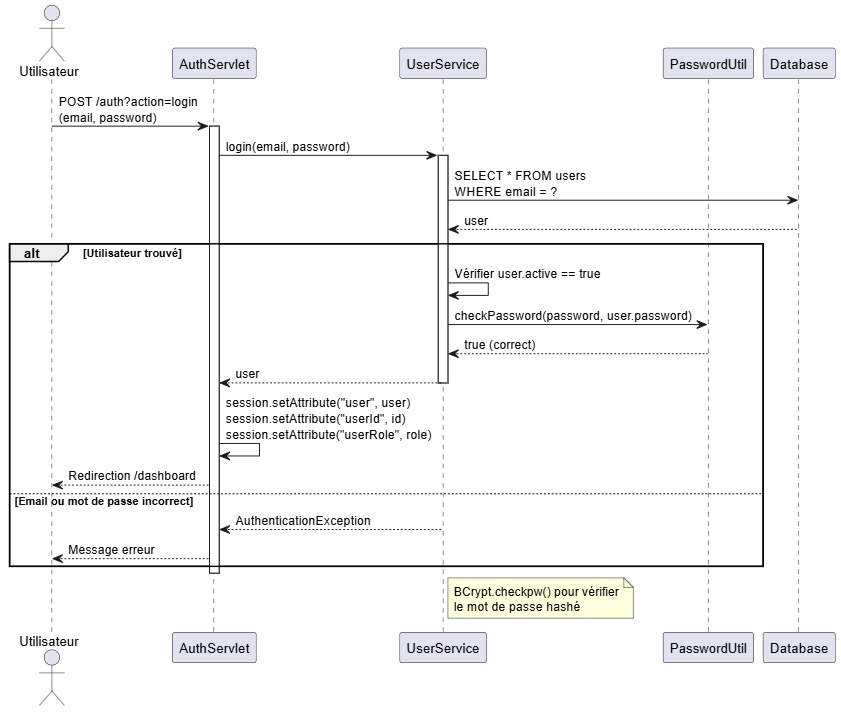
\includegraphics[width=0.95\textwidth]{diagrams/diagrammeSequenceConnexion.jpeg}
\caption{Diagramme de séquence : Connexion}
\label{fig:seq-login}
\end{figure}

\textbf{Description du scénario :}

\begin{enumerate}
    \item L'utilisateur saisit les critères de recherche (destination, date, classe).
    \item Le formulaire soumet une requête GET vers SearchViewController.
    \item Le servlet appelle SearchService avec les critères de recherche.
    \item SearchService utilise FlightDAO pour interroger la base de données.
    \item FlightDAO exécute une requête SQL SELECT avec les critères fournis.
    \item La base retourne les vols correspondants.
    \item FlightDAO construit une liste d'objets Flight et la retourne.
    \item SearchService retourne la liste au servlet.
    \item Le servlet stocke la liste dans les attributs de la requête.
    \item Forward vers la JSP d'affichage des résultats.
    \item Affichage de la liste des vols trouvés à l'utilisateur.
\end{enumerate}

\clearpage

\textbf{Diagramme de séquence 3 : Création de réservation avec paiement (Transaction atomique)}

\begin{figure}[H]
\centering
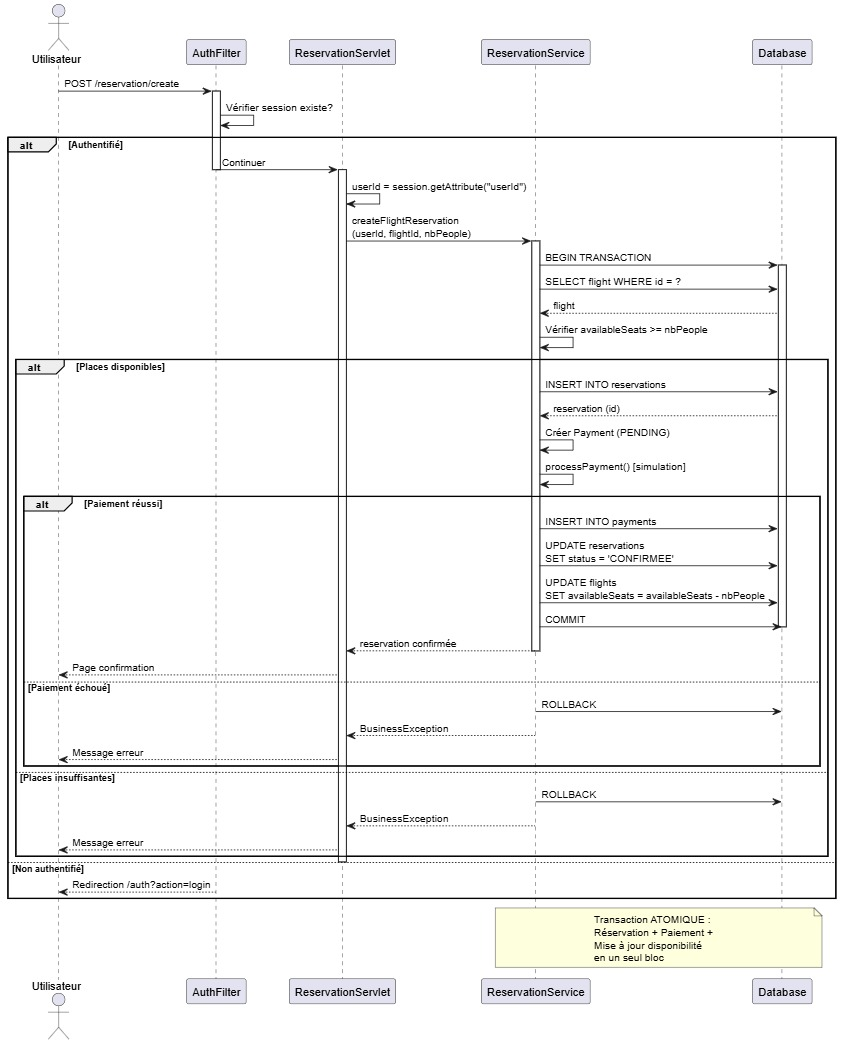
\includegraphics[width=0.98\textwidth]{diagrams/diagrameSequenceReservation.jpeg}
\caption{Diagramme de séquence : Réservation avec paiement (Transaction atomique)}
\label{fig:seq-reservation}
\end{figure}

\textbf{Description du scénario (Transaction ACID) :}

\begin{enumerate}
    \item L'utilisateur confirme sa réservation et ses informations de paiement.
    \item ReservationConfirmServlet reçoit la requête POST.
    \item Le servlet appelle ReservationService pour créer la réservation.
    \item \textbf{Début de transaction JPA} : Toutes les opérations suivantes font partie d'une transaction atomique.
    \item Vérification de l'existence de l'utilisateur.
    \item Vérification de l'existence du vol.
    \item Vérification de la disponibilité des places demandées.
    \item Création de l'objet Reservation avec toutes les informations.
    \item ReservationDAO persiste la réservation en base de données.
    \item La base retourne l'ID de la réservation créée.
    \item La réservation sauvegardée est retournée au service.
    \item Création de l'objet Payment lié à la réservation.
    \item PaymentDAO persiste le paiement en base de données.
    \item La base retourne l'ID du paiement créé.
    \item Le paiement sauvegardé est retourné au service.
    \item \textbf{Commit de la transaction} : Si toutes les étapes ont réussi, la transaction est validée définitivement. En cas d'erreur à n'importe quelle étape, un rollback annule toutes les modifications.
    \item Le service retourne une confirmation de succès au servlet.
    \item Redirection vers la page de confirmation de réservation.
    \item Affichage de la confirmation avec le numéro de réservation.
\end{enumerate}

\textbf{Point clé} : La réservation et le paiement sont créés au sein d'une même transaction JPA. Si le paiement échoue, la réservation est automatiquement annulée (rollback), garantissant ainsi l'intégrité des données.



% ========================================
% CHAPITRE 2 : MÉTHODOLOGIE (Suite)
% ========================================



\section{Développement du projet}

\subsection{Choix technologiques et justifications}

\begin{table}[H]
\centering
\caption{Technologies utilisées dans VoyageConnect}
\label{tab:technologies}
\begin{tabular}{|l|l|p{6cm}|}
\hline
\textbf{Catégorie} & \textbf{Technologie} & \textbf{Justification} \\
\hline
Langage & Java 11 & Robustesse, portabilité, écosystème mature \\
\hline
Framework web & Java EE (Servlets, JSP) & Standard industriel, architecture MVC native \\
\hline
ORM & JPA / Hibernate & Abstraction de la persistance, requêtes JPQL \\
\hline
Base de données & MySQL 8.0 & Fiabilité, support transactionnel (InnoDB) \\
\hline
Serveur d'application & Apache Tomcat 9 & Légèreté, compatibilité, gratuit \\
\hline
Frontend & Bootstrap 5 & Responsive design, composants UI prêts à l'emploi \\
\hline
Gestion versions & Git / GitHub & Traçabilité des modifications, sauvegarde \\
\hline
IDE & VS Code & Léger, extensible, excellent support Java \\
\hline
Build & Maven 3 & Gestion des dépendances, automatisation compilation \\
\hline
\end{tabular}
\end{table}

\subsection{Organisation du code source}

L'organisation du code suit une structure Maven standard avec séparation stricte des couches MVC :

\begin{verbatim}
src/
+-- main/
    +-- java/
        +-- com/voyageconnect/
            +-- controller/        (12 Servlets)
            |   +-- AuthServlet.java
            |   +-- ReservationServlet.java
            |   +-- SearchViewController.java
            |   +-- ...
            +-- dao/               (10 DAOs)
            |   +-- GenericDAO.java
            |   +-- UserDAO.java
            |   +-- ReservationDAO.java
            |   +-- ...
            +-- model/             (15 Entites + Enums)
            |   +-- User.java
            |   +-- Reservation.java
            |   +-- Flight.java
            |   +-- ...
            +-- service/           (5 Services)
            |   +-- UserService.java
            |   +-- ReservationService.java
            |   +-- ...
            +-- filter/            (3 Filtres)
            |   +-- AuthenticationFilter.java
            |   +-- AdminAuthorizationFilter.java
            |   +-- EncodingFilter.java
            +-- util/              (Utilitaires)
            |   +-- JPAUtil.java
            |   +-- PasswordUtil.java
            |   +-- ValidationUtil.java
            +-- exception/         (Exceptions metier)
                +-- BusinessException.java
    +-- resources/
    |   +-- META-INF/
    |       +-- persistence.xml    (Configuration JPA)
    +-- webapp/
        +-- WEB-INF/
        |   +-- web.xml            (Descripteur de deploiement)
        |   +-- views/             (Pages JSP)
        |       +-- user/
        |       |   +-- dashboard.jsp
        |       |   +-- profile.jsp
        |       +-- admin/
        |       +-- reservation/
        |       +-- common/
        |           +-- navbar.jsp
        |           +-- footer.jsp
        +-- css/
        |   +-- style.css
        +-- js/
        +-- index.jsp
+-- test/
    +-- java/                      (Tests unitaires - a implementer)
\end{verbatim}

\subsection{Gestion des transactions avec JPA}

La gestion transactionnelle est cruciale pour garantir l'intégrité des données, en particulier pour les opérations de réservation.

\subsubsection{Configuration JPA}

Le fichier \texttt{persistence.xml} configure l'unité de persistance :

\begin{itemize}
    \item \textbf{Provider} : Hibernate 5.6.x
    \item \textbf{Dialecte} : MySQL8Dialect
    \item \textbf{Propriétés} :
    \begin{itemize}
        \item \texttt{hibernate.hbm2ddl.auto = update} : Mise à jour automatique du schéma
        \item \texttt{hibernate.show\_sql = true} : Affichage des requêtes SQL (développement)
        \item \texttt{hibernate.format\_sql = true} : Formatage des requêtes pour lisibilité
    \end{itemize}
\end{itemize}

\subsubsection{Transactions atomiques dans ReservationService}

Exemple de transaction garantissant l'atomicité de la réservation et du paiement :

\textit{Principe :} Si le paiement échoue, la réservation est annulée automatiquement (rollback). Si toutes les opérations réussissent, elles sont validées ensemble (commit).

\textbf{Étapes de la transaction :}

\begin{enumerate}
    \item Début de transaction (\texttt{em.getTransaction().begin()})
    \item Vérification de l'utilisateur
    \item Vérification du vol et de sa disponibilité
    \item Création de l'entité Reservation
    \item Persistance de la réservation (\texttt{em.persist(reservation)})
    \item Mise à jour du nombre de places disponibles
    \item Création de l'entité Payment
    \item Persistance du paiement (\texttt{em.persist(payment)})
    \item Commit de la transaction (\texttt{em.getTransaction().commit()})
    \item En cas d'erreur à n'importe quelle étape : Rollback (\texttt{em.getTransaction().rollback()})
\end{enumerate}

Ce mécanisme garantit que le système ne se retrouve jamais avec une réservation sans paiement ou un paiement sans réservation.

\subsection{Gestion des sessions et sécurité}

\subsubsection{Authentification et sessions HTTP}

L'authentification repose sur les sessions HTTP de Java EE :

\begin{itemize}
    \item Lors d'une connexion réussie, l'objet \texttt{User} est stocké dans la session : \texttt{session.setAttribute("user", user)}.
    \item Les pages protégées vérifient la présence de cet attribut.
    \item Déconnexion : invalidation de la session (\texttt{session.invalidate()}).
\end{itemize}

\subsubsection{Filtres de sécurité}

\textbf{AuthenticationFilter} : Intercepte toutes les requêtes vers \texttt{/user/*} et \texttt{/reservation/*}. Si l'utilisateur n'est pas connecté, redirection vers la page de login.

\textbf{AdminAuthorizationFilter} : Intercepte les requêtes vers \texttt{/admin/*}. Vérifie que l'utilisateur connecté a le rôle ADMIN, sinon erreur 403.

\textbf{EncodingFilter} : Force l'encodage UTF-8 pour toutes les requêtes/réponses, évitant les problèmes d'affichage des caractères accentués.

\subsubsection{Hachage des mots de passe}

Les mots de passe ne sont jamais stockés en clair. Ils sont hachés avec l'algorithme BCrypt avant insertion en base de données.

\textbf{Lors de l'inscription :}
\begin{enumerate}
    \item L'utilisateur saisit son mot de passe.
    \item BCrypt génère un hash sécurisé.
    \item Le hash est stocké dans \texttt{users.password}.
\end{enumerate}

\textbf{Lors de l'authentification :}
\begin{enumerate}
    \item L'utilisateur saisit son mot de passe.
    \item BCrypt compare le mot de passe saisi avec le hash stocké.
    \item Authentification réussie si correspondance.
\end{enumerate}

% ========================================
% CHAPITRE 3 : RÉALISATION TECHNIQUE
% ========================================

\chapter{Réalisation technique}

\section{Mise en œuvre du projet}

\subsection{Environnement de développement}

\subsubsection{Configuration initiale}

La mise en place de l'environnement de développement a nécessité l'installation et la configuration des composants suivants :

\begin{enumerate}
    \item \textbf{JDK 11} (Amazon Corretto) : Installation du kit de développement Java.
    \item \textbf{Apache Tomcat 9.0.113} : Téléchargement et configuration du serveur d'applications.
    \item \textbf{MySQL 8.0} : Installation du SGBD et création de la base de données \texttt{voyageconnect\_db}.
    \item \textbf{Apache Maven 3.8+} : Gestionnaire de build et de dépendances.
    \item \textbf{VS Code} avec extensions Java : IDE principal avec support Servlet/JSP.
    \item \textbf{Git} : Système de contrôle de version.
\end{enumerate}

\subsubsection{Configuration de la base de données}

Création de la base de données et d'un utilisateur dédié :

\begin{verbatim}
CREATE DATABASE voyageconnect_db 
  CHARACTER SET utf8mb4 
  COLLATE utf8mb4_unicode_ci;

CREATE USER 'voyageconnect_user'@'localhost' 
  IDENTIFIED BY 'secure_password';

GRANT ALL PRIVILEGES ON voyageconnect_db.* 
  TO 'voyageconnect_user'@'localhost';

FLUSH PRIVILEGES;
\end{verbatim}

La base utilise le moteur InnoDB pour le support des transactions ACID et des clés étrangères.

\subsection{Architecture de la couche Modèle}

\subsubsection{Entités JPA principales}

\textbf{Entité User (utilisateur)}

Cette entité représente un utilisateur du système (client ou administrateur).

\textit{Caractéristiques principales :}
\begin{itemize}
    \item Hachage sécurisé des mots de passe avec BCrypt
    \item Support de deux rôles : USER et ADMIN (énumération \texttt{UserRole})
    \item Relation bidirectionnelle avec Reservation (1..N)
    \item Horodatage automatique de création et modification
\end{itemize}

\textit{Annotations JPA clés :}
\begin{itemize}
    \item \texttt{@Entity} : Déclare la classe comme entité persistante
    \item \texttt{@Column(unique = true)} : Email unique dans la base
    \item \texttt{@Enumerated(EnumType.STRING)} : Stockage du rôle en chaîne
    \item \texttt{@OneToMany(mappedBy = "user")} : Collection de réservations
\end{itemize}

\textbf{Entité Reservation}

Entité centrale du système, gérant toutes les réservations.

\textit{Points clés :}
\begin{itemize}
    \item Type de réservation polymorphe : FLIGHT, HOTEL ou CIRCUIT
    \item Relations conditionnelles : un seul des attributs \texttt{flight}, \texttt{hotel}, \texttt{circuit} est non-null
    \item Relation obligatoire avec User (ManyToOne)
    \item Relation bijective avec Payment (OneToOne)
    \item Gestion de statut : EN\_ATTENTE, CONFIRMEE, ANNULEE
    \item Génération automatique d'un numéro de réservation unique (format: RES-YYYYMMDD-XXXXX)
\end{itemize}

\textit{Logique métier :}
\begin{itemize}
    \item Calcul automatique du montant total selon le type et le nombre de personnes
    \item Vérification de disponibilité avant persistance
    \item Validation des dates (check-in < check-out pour hôtels)
\end{itemize}

\textbf{Entité Payment}

Gère les transactions de paiement.

\textit{Caractéristiques :}
\begin{itemize}
    \item Relation OneToOne obligatoire avec Reservation
    \item Génération de numéro de transaction unique (format: TXN-YYYYMMDD-XXXXX)
    \item Support de plusieurs méthodes de paiement : CARD, PAYPAL, BANK\_TRANSFER
    \item Statuts possibles: PENDING, COMPLETED, FAILED, REFUNDED
    \item Horodatage de la transaction
\end{itemize}

\textbf{Entités de services (Flight, Hotel, Circuit)}

Ces trois entités représentent les services réservables.

\textit{Attributs communs :}
\begin{itemize}
    \item Lien obligatoire vers une Destination (ManyToOne)
    \item Prix (type DECIMAL pour précision monétaire)
    \item Disponibilité (places ou chambres)
    \item Descriptions textuelles
\end{itemize}

\textit{Spécificités :}
\begin{itemize}
    \item \textbf{Flight} : Numéro de vol, compagnie, dates de départ/arrivée, classe (ECONOMY/BUSINESS/FIRST)
    \item \textbf{Hotel} : Nombre d'étoiles (1-5), équipements (wifi, piscine, restaurant, parking)
    \item \textbf{Circuit} : Durée en jours, itinéraire, niveau de difficulté
\end{itemize}

\subsection{Architecture de la couche DAO}

\subsubsection{Pattern DAO générique}

Pour éviter la duplication de code CRUD, une classe abstraite \texttt{GenericDAO<T>} a été créée.

\textit{Méthodes fournies :}
\begin{itemize}
    \item \texttt{persist(T entity)} : Insertion en base
    \item \texttt{findById(Long id)} : Récupération par identifiant
    \item \texttt{findAll()} : Liste de toutes les entités
    \item \texttt{update(T entity)} : Mise à jour
    \item \texttt{delete(T entity)} : Suppression
\end{itemize}

Chaque DAO spécifique (ex: \texttt{UserDAO}, \texttt{FlightDAO}) hérite de \texttt{GenericDAO} et ajoute des méthodes métier.

\subsubsection{UserDAO - Méthodes spécialisées}

\texttt{findByEmail(String email)} : Recherche un utilisateur par email (login).

\textit{Requête JPQL :}
\begin{verbatim}
SELECT u FROM User u WHERE u.email = :email
\end{verbatim}

\texttt{authenticate(String email, String password)} : Vérifie les identifiants avec BCrypt.

\textit{Logique :}
\begin{enumerate}
    \item Rechercher l'utilisateur par email
    \item Si trouvé, comparer le hash du mot de passe avec \texttt{BCrypt.checkpw()}
    \item Retourner l'utilisateur si succès, sinon null
\end{enumerate}

\subsubsection{ReservationDAO - Requêtes complexes}

\texttt{findByUserId(Long userId)} : Toutes les réservations d'un utilisateur.

\begin{verbatim}
SELECT r FROM Reservation r WHERE r.user.id = :userId 
ORDER BY r.createdAt DESC
\end{verbatim}

\texttt{findByStatus(ReservationStatus status)} : Recherche par statut.

\texttt{findPendingReservations()} : Réservations en attente (pour monitoring).

\subsubsection{FlightDAO - Recherche multicritère}

\texttt{searchFlights(String departureCity, String arrivalCity, Date date)}

\begin{verbatim}
SELECT f FROM Flight f WHERE 
  (:departureCity IS NULL OR f.departureCity LIKE :departureCity) AND
  (:arrivalCity IS NULL OR f.destination.city LIKE :arrivalCity) AND
  (:date IS NULL OR f.departureDate = :date) AND
  f.availableSeats > 0
ORDER BY f.price ASC
\end{verbatim}

Cette requête permet une recherche flexible avec paramètres optionnels.

\subsection{Architecture de la couche Service}

\subsubsection{UserService - Gestion des utilisateurs}

\texttt{register(User user)} : Inscription d'un nouvel utilisateur.

\textit{Étapes :}
\begin{enumerate}
    \item Valider les données (email valide, mot de passe fort)
    \item Vérifier que l'email n'est pas déjà utilisé
    \item Hacher le mot de passe avec BCrypt
    \item Définir le rôle par défaut (USER) et statut actif
    \item Persister l'utilisateur
\end{enumerate}

\texttt{login(String email, String password)} : Authentification.

\textit{Retourne :}
\begin{itemize}
    \item L'objet User si authentification réussie
    \item null si échec (identifiants incorrects ou compte inactif)
\end{itemize}

\subsubsection{ReservationService - Logique métier complexe}

\texttt{createFlightReservation(User user, Flight flight, int numberOfPeople)}

\textit{Transaction ACID en 8 étapes :}

\begin{enumerate}
    \item Début de transaction
    \item Vérifier disponibilité du vol (\texttt{availableSeats >= numberOfPeople})
    \item Calculer montant total (\texttt{flight.price * numberOfPeople})
    \item Créer objet Reservation avec statut EN\_ATTENTE
    \item Générer numéro de réservation unique
    \item Persister la réservation
    \item Mettre à jour \texttt{flight.availableSeats}
    \item Créer et persister Payment avec statut PENDING
    \item Commit de la transaction
    \item En cas d'erreur : rollback automatique
\end{enumerate}

\textit{Garantie d'atomicité :} Si n'importe quelle étape échoue (ex: plus de places disponibles entre la vérification et la persistance), toute la transaction est annulée.

\texttt{confirmReservation(Long reservationId)}

Met à jour le statut de la réservation à CONFIRMEE et le paiement à COMPLETED.

\texttt{cancelReservation(Long reservationId)}

\textit{Actions :}
\begin{itemize}
    \item Mettre le statut à ANNULEE
    \item Restaurer les places disponibles (pour vols/circuits)
    \item Mettre le paiement en statut REFUNDED
\end{itemize}

\subsection{Architecture de la couche Contrôleur}

\subsubsection{AuthServlet - Gestion de l'authentification}

\textbf{URL :} \texttt{/auth}

\textbf{Méthodes HTTP supportées :}

\texttt{doGet()} : Affiche la page de connexion (\texttt{login.jsp}).

\texttt{doPost()} : Traite la soumission du formulaire de connexion.

\textit{Workflow :}
\begin{enumerate}
    \item Récupérer email et password depuis la requête
    \item Appeler \texttt{UserService.login(email, password)}
    \item Si authentification réussie :
    \begin{itemize}
        \item Créer une session HTTP
        \item Stocker l'objet User dans la session
        \item Rediriger vers le dashboard approprié (user ou admin)
    \end{itemize}
    \item Si échec : retourner à login.jsp avec message d'erreur
\end{enumerate}

\subsubsection{SearchViewController - Recherche de services}

\textbf{URL :} \texttt{/search}

\textbf{Paramètres supportés :}
\begin{itemize}
    \item \texttt{type} : Type de recherche (flight, hotel, circuit)
    \item \texttt{departureCity}, \texttt{arrivalCity} : Critères de vol
    \item \texttt{date} : Date de départ/arrivée
    \item \texttt{destination} : Destination pour hôtels/circuits
    \item \texttt{stars} : Étoiles pour hôtels
\end{itemize}

\texttt{doGet()} : Affiche le formulaire de recherche.

\texttt{doPost()} : Traite la recherche.

\textit{Exemple pour recherche de vols :}
\begin{enumerate}
    \item Récupérer les paramètres de recherche
    \item Appeler \texttt{FlightDAO.searchFlights()}
    \item Stocker les résultats dans la requête (\texttt{request.setAttribute("flights", flights)})
    \item Forward vers \texttt{search-results.jsp}
\end{enumerate}

\subsubsection{ReservationConfirmServlet - Finalisation de réservation}

\textbf{URL :} \texttt{/reservation/confirm}

\textbf{Workflow de réservation :}

\begin{enumerate}
    \item \textbf{Étape 1 - Sélection du service} : L'utilisateur clique sur "Réserver" depuis les résultats de recherche.
    
    \item \textbf{Étape 2 - Formulaire de confirmation} : \texttt{ReservationNewServlet} affiche un formulaire avec :
    \begin{itemize}
        \item Détails du service sélectionné
        \item Nombre de personnes
        \item Dates (pour hôtels)
        \item Récapitulatif du prix
    \end{itemize}
    
    \item \textbf{Étape 3 - Validation et paiement} : \texttt{ReservationConfirmServlet.doPost()} :
    \begin{itemize}
        \item Récupère l'utilisateur de la session
        \item Récupère le service à réserver (vol/hôtel/circuit)
        \item Appelle \texttt{ReservationService.createReservation()} (transaction atomique)
        \item Si succès : redirection vers \texttt{/reservation/success?reservationNumber=XXX}
        \item Si échec : retour au formulaire avec message d'erreur
    \end{itemize}
    
    \item \textbf{Étape 4 - Confirmation} : \texttt{ReservationSuccessServlet} affiche :
    \begin{itemize}
        \item Numéro de réservation
        \item Récapitulatif complet
        \item Numéro de transaction de paiement
        \item Lien vers le tableau de bord
    \end{itemize}
\end{enumerate}

\subsubsection{AdminServlet - Gestion du catalogue}

\textbf{URL :} \texttt{/admin/catalog}

\textbf{Actions supportées :}

\texttt{action=listFlights} : Liste tous les vols avec options d'édition/suppression.

\texttt{action=addFlight} : Affiche le formulaire d'ajout de vol.

\texttt{action=editFlight\&id=X} : Formulaire de modification d'un vol.

\texttt{action=deleteFlight\&id=X} : Suppression d'un vol (avec vérification : impossible si réservations actives).

\textit{Même logique pour hôtels et circuits.}

\subsection{Interfaces utilisateur (Vue)}

\subsubsection{Structure des pages JSP}

Utilisation du pattern \textbf{Template} pour éviter la duplication :

\begin{itemize}
    \item \texttt{common/header.jsp} : En-tête HTML, meta tags, liens CSS
    \item \texttt{common/navbar.jsp} : Barre de navigation (différente selon rôle)
    \item \texttt{common/footer.jsp} : Pied de page avec liens et copyright
\end{itemize}

Chaque page JSP inclut ces composants :
\begin{verbatim}
<%@ include file="/WEB-INF/views/common/header.jsp" %>
<%@ include file="/WEB-INF/views/common/navbar.jsp" %>

<!-- Contenu spécifique de la page -->

<%@ include file="/WEB-INF/views/common/footer.jsp" %>
\end{verbatim}

\subsubsection{Dashboard utilisateur}

\textbf{Fichier :} \texttt{user/dashboard.jsp}

\textbf{Sections principales :}

\begin{enumerate}
    \item \textbf{En-tête de bienvenue} : "Bienvenue, [Prénom] [Nom]" avec photo de profil par défaut.
    
    \item \textbf{Statistiques personnelles} :
    \begin{itemize}
        \item Nombre total de réservations
        \item Réservations actives (confirmées)
        \item Réservations en attente
        \item Montant total dépensé
    \end{itemize}
    
    \item \textbf{Tableau des réservations récentes} :
    \begin{itemize}
        \item Numéro de réservation
        \item Type (Vol/Hôtel/Circuit)
        \item Destination
        \item Date de création
        \item Montant total
        \item Statut (badge coloré : vert=confirmée, orange=en attente, rouge=annulée)
        \item Actions : Voir détails, Annuler (si confirmée)
    \end{itemize}
    
    \item \textbf{Boutons d'actions rapides} :
    \begin{itemize}
        \item Nouvelle recherche
        \item Voir toutes les réservations
        \item Modifier le profil
    \end{itemize}
\end{enumerate}

\textbf{Technologies utilisées :}
\begin{itemize}
    \item JSTL pour itération sur les réservations (\texttt{<c:forEach>})
    \item Bootstrap pour le design responsive (cards, badges, tables)
    \item JavaScript pour confirmations d'annulation
\end{itemize}

\subsubsection{Page de recherche}

\textbf{Fichier :} \texttt{search/index.jsp}

\textbf{Fonctionnalités :}

\begin{enumerate}
    \item \textbf{Onglets de sélection} : Vols | Hôtels | Circuits (tabs Bootstrap).
    
    \item \textbf{Formulaire de recherche de vols} :
    \begin{itemize}
        \item Ville de départ (autocomplete avec destinations en DB)
        \item Ville d'arrivée
        \item Date de départ (datepicker)
        \item Nombre de passagers
        \item Classe (Économique/Affaires/Première)
    \end{itemize}
    
    \item \textbf{Formulaire de recherche d'hôtels} :
    \begin{itemize}
        \item Destination
        \item Date d'arrivée / Date de départ
        \item Nombre de chambres
        \item Nombre d'étoiles (filtre min-max)
        \item Équipements (checkboxes : Wi-Fi, Piscine, Restaurant)
    \end{itemize}
    
    \item \textbf{Affichage des résultats} :
    \begin{itemize}
        \item Cards Bootstrap avec image, titre, prix, caractéristiques
        \item Tri par : Prix croissant/décroissant, Date, Popularité
        \item Filtres dynamiques (JavaScript) : Prix max, Étoiles, Équipements
        \item Pagination (10 résultats par page)
        \item Bouton "Réserver" sur chaque résultat
    \end{itemize}
\end{enumerate}

\subsubsection{Interface d'administration}

\textbf{Fichier principal :} \texttt{admin/dashboard.jsp}

\textbf{Menu latéral avec sections :}

\begin{enumerate}
    \item \textbf{Tableau de bord} : Statistiques globales
    \begin{itemize}
        \item Nombre total de réservations ce mois
        \item Chiffre d'affaires total
        \item Nombre d'utilisateurs inscrits
        \item Taux d'occupation moyen (vols/hôtels)
    \end{itemize}
    
    \item \textbf{Gestion des vols} :
    \begin{itemize}
        \item Liste avec tableau DataTables (recherche, tri, pagination)
        \item Colonnes : Numéro, Compagnie, Départ, Arrivée, Prix, Places disponibles, Actions
        \item Actions : Éditer (modal), Supprimer (confirmation), Dupliquer
        \item Bouton "Ajouter un vol" : formulaire modal avec tous les champs
    \end{itemize}
    
    \item \textbf{Gestion des hôtels} : Structure similaire aux vols.
    
    \item \textbf{Gestion des circuits} : Structure similaire.
    
    \item \textbf{Gestion des utilisateurs} :
    \begin{itemize}
        \item Liste de tous les utilisateurs
        \item Filtres : Rôle (USER/ADMIN), Statut (Actif/Inactif)
        \item Actions : Voir profil, Désactiver/Activer compte, Changer rôle
    \end{itemize}
    
    \item \textbf{Toutes les réservations} :
    \begin{itemize}
        \item Vue globale avec filtres (Statut, Type, Période)
        \item Export CSV pour analyse
    \end{itemize}
\end{enumerate}

\section{Fonctionnalités implémentées}

\subsection{Gestion des utilisateurs}

\subsubsection{Inscription}

\textbf{URL :} \texttt{/register}

\textit{Formulaire :}
\begin{itemize}
    \item Prénom, Nom
    \item Email (vérifié avec regex)
    \item Mot de passe (minimum 8 caractères, avec confirmation)
    \item Téléphone (optionnel)
    \item Adresse (optionnelle)
\end{itemize}

\textit{Validations :}
\begin{itemize}
    \item Email unique (vérification en base)
    \item Mot de passe fort (lettres, chiffres, caractères spéciaux)
    \item Concordance mot de passe / confirmation
\end{itemize}

\textit{Flux :}
\begin{enumerate}
    \item Soumission du formulaire
    \item Validation côté client (JavaScript)
    \item Validation côté serveur (Servlet)
    \item Hachage du mot de passe (BCrypt)
    \item Persistance en base de données
    \item Connexion automatique
    \item Redirection vers le dashboard
\end{enumerate}

\subsubsection{Connexion et déconnexion}

\textbf{Connexion :}
\begin{itemize}
    \item URL : \texttt{/auth?action=login}
    \item Authentification par email/mot de passe
    \item Création de session HTTP
    \item Timeout de session : 30 minutes d'inactivité
\end{itemize}

\textbf{Déconnexion :}
\begin{itemize}
    \item URL : \texttt{/auth?action=logout}
    \item Invalidation de la session
    \item Redirection vers la page d'accueil
\end{itemize}

\subsubsection{Gestion de profil}

\textbf{URL :} \texttt{/user/profile}

\textit{Fonctionnalités :}
\begin{itemize}
    \item Affichage des informations personnelles
    \item Modification : Nom, Prénom, Téléphone, Adresse
    \item Changement de mot de passe : Mot de passe actuel + Nouveau + Confirmation
    \item Upload de photo de profil (fonctionnalité future)
\end{itemize}

\subsection{Recherche de services}

\subsubsection{Recherche de vols}

\textit{Critères supportés :}
\begin{itemize}
    \item Ville de départ (obligatoire)
    \item Ville d'arrivée (obligatoire)
    \item Date de départ (obligatoire)
    \item Nombre de passagers (défaut : 1)
    \item Classe (Économique, Affaires, Première - optionnel)
\end{itemize}

\textit{Affichage des résultats :}
\begin{itemize}
    \item Numéro de vol
    \item Compagnie aérienne (avec logo si disponible)
    \item Horaires de départ et d'arrivée
    \item Durée du vol (calculée)
    \item Prix par personne
    \item Nombre de places restantes
    \item Classe disponible
    \item Badge "Bonne affaire" si prix inférieur à la moyenne
    \item Bouton "Sélectionner"
\end{itemize}

\subsubsection{Recherche d'hôtels}

\textit{Critères :}
\begin{itemize}
    \item Destination (obligatoire)
    \item Date d'arrivée / Date de départ (obligatoires)
    \item Nombre d'étoiles minimum (1-5)
    \item Équipements : Wi-Fi, Piscine, Restaurant, Parking
    \item Prix maximum par nuit
\end{itemize}

\textit{Résultats :}
\begin{itemize}
    \item Nom de l'hôtel
    \item Adresse complète
    \item Étoiles (affichées avec icônes)
    \item Prix par nuit
    \item Équipements disponibles (icônes)
    \item Note moyenne (si des avis existent)
    \item Photo principale
    \item Bouton "Voir détails" + "Réserver"
\end{itemize}

\subsubsection{Recherche de circuits}

\textit{Critères :}
\begin{itemize}
    \item Destination
    \item Durée minimum/maximum (en jours)
    \item Période souhaitée
    \item Budget maximum
\end{itemize}

\textit{Résultats :}
\begin{itemize}
    \item Nom du circuit
    \item Itinéraire (villes visitées)
    \item Durée (jours/nuits)
    \item Prix par personne
    \item Dates de départ disponibles
    \item Niveau de difficulté
    \item Inclus : Hébergement, Repas, Transport, Guide
    \item Places disponibles
\end{itemize}

\subsection{Système de réservation}

\subsubsection{Processus de réservation}

\textbf{Étape 1 : Sélection du service}

Depuis les résultats de recherche, l'utilisateur clique sur "Réserver".

\textbf{Étape 2 : Formulaire de détails}

Page \texttt{reservation/new.jsp} affiche :
\begin{itemize}
    \item Récapitulatif du service sélectionné
    \item Formulaire avec :
    \begin{itemize}
        \item Nombre de personnes (défaut : 1, max : places disponibles)
        \item Dates (pour hôtels : check-in / check-out)
        \item Informations complémentaires (demandes spéciales)
    \end{itemize}
    \item Calcul dynamique du prix total (JavaScript)
\end{itemize}

\textbf{Étape 3 : Confirmation et paiement}

Page \texttt{reservation/confirm.jsp} affiche :
\begin{itemize}
    \item Récapitulatif complet
    \item Détails du voyageur (pré-remplis depuis le profil)
    \item Choix de la méthode de paiement (Carte bancaire, PayPal, Virement)
    \item Case à cocher "J'accepte les conditions générales"
    \item Bouton "Confirmer et payer"
\end{itemize}

\textbf{Traitement (ReservationConfirmServlet) :}
\begin{enumerate}
    \item Vérification de disponibilité en temps réel
    \item Transaction atomique :
    \begin{itemize}
        \item Création de la réservation (statut EN\_ATTENTE)
        \item Décrémentation du nombre de places disponibles
        \item Création du paiement (statut PENDING)
    \end{itemize}
    \item Simulation de traitement de paiement (succès par défaut)
    \item Si succès :
    \begin{itemize}
        \item Mise à jour statut réservation → CONFIRMEE
        \item Mise à jour statut paiement → COMPLETED
        \item Commit de la transaction
    \end{itemize}
    \item Si échec :
    \begin{itemize}
        \item Rollback de la transaction
        \item Message d'erreur à l'utilisateur
    \end{itemize}
\end{enumerate}

\textbf{Étape 4 : Page de succès}

Page \texttt{reservation/success.jsp} affiche :
\begin{itemize}
    \item Message de confirmation
    \item Numéro de réservation (format : RES-20250127-12345)
    \item Numéro de transaction (format : TXN-20250127-67890)
    \item Récapitulatif complet
    \item Conseils : "Imprimez ce récapitulatif", "Arrivez 2h avant le départ", etc.
    \item Boutons : "Retour au dashboard", "Voir mes réservations"
\end{itemize}

\subsubsection{Annulation de réservation}

\textbf{Conditions :}
\begin{itemize}
    \item Seules les réservations avec statut CONFIRMEE peuvent être annulées
    \item Annulation possible jusqu'à 24h avant la date de service
\end{itemize}

\textbf{Processus :}
\begin{enumerate}
    \item Utilisateur clique sur "Annuler" depuis le dashboard
    \item Fenêtre de confirmation JavaScript : "Êtes-vous sûr ?"
    \item Requête POST vers \texttt{/reservation/cancel?id=XXX}
    \item Servlet vérifie les conditions d'annulation
    \item Si autorisé :
    \begin{itemize}
        \item Mise à jour statut réservation → ANNULEE
        \item Restauration des places disponibles
        \item Mise à jour statut paiement → REFUNDED
        \item Message : "Votre réservation a été annulée. Le remboursement sera effectué sous 7-10 jours."
    \end{itemize}
    \item Si refusé : Message d'erreur avec raison
\end{enumerate}

\subsection{Tableau de bord utilisateur}

\subsubsection{Vue d'ensemble}

Le dashboard utilisateur (\texttt{/user/dashboard}) est la page centrale après connexion.

\textbf{Composants :}

\begin{enumerate}
    \item \textbf{Barre de bienvenue}
    \begin{itemize}
        \item "Bonjour, [Prénom]"
        \item Date et heure actuelles
        \item Photo de profil (ou initiales si non uploadée)
    \end{itemize}
    
    \item \textbf{Cartes statistiques (4 cards)}
    \begin{itemize}
        \item Total de réservations (icône : valise)
        \item Réservations actives (icône : check vert)
        \item Réservations en attente (icône : horloge orange)
        \item Montant total dépensé (icône : euro)
    \end{itemize}
    
    \item \textbf{Tableau des réservations récentes (5 dernières)}
    \begin{itemize}
        \item Colonnes : Numéro, Type, Service, Date, Montant, Statut, Actions
        \item Badge de statut coloré
        \item Actions : Voir détails (icône œil), Annuler (icône poubelle)
    \end{itemize}
    
    \item \textbf{Graphique (optionnel, avec Chart.js)}
    \begin{itemize}
        \item Évolution des réservations par mois
        \item Répartition par type de service (diagramme en camembert)
    \end{itemize}
    
    \item \textbf{Boutons d'actions rapides}
    \begin{itemize}
        \item "Rechercher un vol"
        \item "Rechercher un hôtel"
        \item "Voir toutes les réservations"
        \item "Modifier mon profil"
    \end{itemize}
\end{enumerate}

\subsubsection{Liste complète des réservations}

\textbf{URL :} \texttt{/reservation/list}

\textit{Fonctionnalités :}
\begin{itemize}
    \item Affichage paginé (20 réservations par page)
    \item Tri par : Date (défaut), Montant, Statut, Type
    \item Filtres :
    \begin{itemize}
        \item Par type (Tous / Vols / Hôtels / Circuits)
        \item Par statut (Tous / Confirmées / En attente / Annulées)
        \item Par période (Ce mois / Ce trimestre / Cette année / Personnalisé)
    \end{itemize}
    \item Recherche par numéro de réservation
    \item Export CSV de l'historique complet
\end{itemize}

\subsection{Interface d'administration}

\subsubsection{Gestion du catalogue de vols}

\textbf{Liste des vols}

URL : \texttt{/admin/flights}

\textit{Tableau avec colonnes :}
\begin{itemize}
    \item ID
    \item Numéro de vol
    \item Compagnie
    \item Départ (ville + date/heure)
    \item Arrivée (ville + date/heure)
    \item Prix
    \item Places totales
    \item Places disponibles
    \item Statut (Actif / Complet / Annulé)
    \item Actions : Éditer, Supprimer, Dupliquer
\end{itemize}

\textbf{Ajout d'un vol}

Formulaire modal avec champs :
\begin{itemize}
    \item Numéro de vol (ex: AF1234)
    \item Compagnie aérienne (select : Air France, Emirates, etc.)
    \item Ville de départ (autocomplete depuis table destinations)
    \item Ville d'arrivée (autocomplete)
    \item Date et heure de départ
    \item Date et heure d'arrivée
    \item Prix en euros
    \item Nombre de places total
    \item Classe (Économique, Affaires, Première)
\end{itemize}

\textit{Validation :}
\begin{itemize}
    \item Date d'arrivée > Date de départ
    \item Prix > 0
    \item Places > 0
    \item Numéro de vol unique
\end{itemize}

\textbf{Modification et suppression}

\textit{Édition :} Formulaire pré-rempli avec données existantes.

\textit{Suppression :}
\begin{itemize}
    \item Vérification : impossible si réservations actives liées
    \item Confirmation : "Ce vol a X réservations confirmées. Êtes-vous sûr ?"
    \item Soft delete : mise à jour du statut à "CANCELLED" (pas de suppression physique)
\end{itemize}

\subsubsection{Statistiques administrateur}

\textbf{Page :} \texttt{/admin/dashboard}

\textit{Métriques affichées :}

\begin{enumerate}
    \item \textbf{Chiffre d'affaires}
    \begin{itemize}
        \item CA total ce mois
        \item CA total cette année
        \item Évolution (% vs mois précédent)
        \item Graphique linéaire des 12 derniers mois
    \end{itemize}
    
    \item \textbf{Réservations}
    \begin{itemize}
        \item Nombre total de réservations
        \item Réservations ce mois
        \item Taux d'annulation (%)
        \item Répartition par type (diagramme en camembert)
    \end{itemize}
    
    \item \textbf{Utilisateurs}
    \begin{itemize}
        \item Nombre total d'utilisateurs
        \item Nouveaux utilisateurs ce mois
        \item Taux de conversion (utilisateurs ayant au moins 1 réservation)
    \end{itemize}
    
    \item \textbf{Taux d'occupation}
    \begin{itemize}
        \item Vols : (Places réservées / Places totales) * 100
        \item Hôtels : Taux de remplissage moyen
        \item Circuits : Taux de participation
    \end{itemize}
    
    \item \textbf{Top services}
    \begin{itemize}
        \item 5 vols les plus réservés
        \item 5 hôtels les plus populaires
        \item 5 destinations préférées
    \end{itemize}
\end{enumerate}

\section{Problèmes rencontrés et solutions}

\subsection{Problèmes techniques}

\subsubsection{Problème 1 : Gestion des transactions JPA}

\textbf{Contexte :} Lors de la création d'une réservation, il arrivait que la réservation soit créée mais pas le paiement, ou vice-versa.

\textbf{Cause :} Utilisation incorrecte des transactions JPA. Les opérations n'étaient pas toutes dans la même transaction.

\textbf{Solution :}
\begin{itemize}
    \item Encapsulation de toutes les opérations liées (réservation + paiement + mise à jour disponibilité) dans un seul bloc transactionnel.
    \item Utilisation de \texttt{try-catch} avec rollback en cas d'exception.
    \item Test de tous les scénarios d'erreur (places insuffisantes, échec de paiement, etc.).
\end{itemize}

\subsubsection{Problème 2 : Encodage des caractères accentués}

\textbf{Symptôme :} Les caractères accentués (e, e, a, c) s'affichaient incorrectement (caracteres illisibles ou points d'interrogation).

\textbf{Cause :} Encodage non defini ou incoherent entre la base de donnees, les JSP et les servlets.

\textbf{Solution :}
\begin{itemize}
    \item Configuration de la base de donnees en UTF-8 avec CHARACTER SET utf8mb4 COLLATE utf8mb4\_unicode\_ci
    \item Ajout de EncodingFilter forcant UTF-8 pour toutes les requetes et reponses
    \item Directive dans chaque JSP avec page contentType text/html charset UTF-8
    \item Configuration du connecteur MySQL avec useUnicode=true et characterEncoding=UTF-8
\end{itemize}

\subsubsection{Problème 3 : Timeout de session}

\textbf{Problème :} Les utilisateurs étaient déconnectés après quelques minutes d'inactivité.

\textbf{Cause :} Timeout de session par défaut de Tomcat trop court (5 minutes).

\textbf{Solution :}
\begin{itemize}
    \item Configuration dans \texttt{web.xml} : \texttt{<session-timeout>30</session-timeout>} (30 minutes)
    \item Implémentation d'un mécanisme "Keep-alive" : requête AJAX toutes les 5 minutes pour maintenir la session active
\end{itemize}

\subsubsection{Problème 4 : Erreurs 404 sur CSS/JS}

\textbf{Symptôme :} Pages JSP s'affichaient sans styles ni scripts.

\textbf{Cause :} Chemins relatifs incorrects dans les includes JSP.

\textbf{Solution :}
\begin{itemize}
    \item Utilisation de chemins absolus avec contexte : \texttt{\${pageContext.request.contextPath}/css/style.css}
    \item Vérification de la structure du dossier \texttt{webapp}
    \item Configuration correcte du mapping des servlets (éviter de mapper \texttt{/*})
\end{itemize}

\subsection{Problèmes de conception}

\subsubsection{Problème : Relations polymorphes (Reservation $\rightarrow$ Flight/Hotel/Circuit)}

\textbf{Défi :} Une réservation peut être liée à un vol, un hôtel OU un circuit, mais pas plusieurs à la fois.

\textbf{Options envisagées :}
\begin{enumerate}
    \item Trois tables séparées : \texttt{flight\_reservations}, \texttt{hotel\_reservations}, \texttt{circuit\_reservations}
    \item Table unique avec trois colonnes FK (\texttt{flight\_id}, \texttt{hotel\_id}, \texttt{circuit\_id}) dont une seule non-null
    \item Héritage JPA (Single Table Strategy)
\end{enumerate}

\textbf{Solution retenue :} Option 2 (table unique avec FKs nullables).

\textit{Justification :}
\begin{itemize}
    \item Simplicité de requêtage (toutes les réservations dans une table)
    \item Facile à étendre (ajout d'un nouveau type = nouvelle colonne FK)
    \item Contrainte applicative dans le Service pour garantir qu'une seule FK est non-null
\end{itemize}

\textit{Contrainte CHECK SQL (non supportée partout) :}
\begin{verbatim}
CHECK (
  (flight_id IS NOT NULL AND hotel_id IS NULL AND circuit_id IS NULL) OR
  (flight_id IS NULL AND hotel_id IS NOT NULL AND circuit_id IS NULL) OR
  (flight_id IS NULL AND hotel_id IS NULL AND circuit_id IS NOT NULL)
)
\end{verbatim}

\subsubsection{Problème : Performance des recherches}

\textbf{Observation :} Recherches de vols lentes avec critères multiples.

\textbf{Optimisations apportées :}
\begin{enumerate}
    \item Ajout d'index composites : \texttt{INDEX(destination\_id, departure\_date)}
    \item Utilisation de requêtes JPQL avec FETCH JOIN pour éviter le problème N+1
    \item Cache de second niveau Hibernate pour les destinations (rarement modifiées)
    \item Pagination des résultats (max 50 résultats par page)
\end{enumerate}

\section{Tests et validation}

\subsection{Scénarios de test complets}

\subsubsection{Scénario 1 : Inscription et première réservation}

\begin{enumerate}
    \item Accès à la page d'accueil
    \item Clic sur "S'inscrire"
    \item Remplissage du formulaire : Jean Dupont, jean.dupont@email.com, mot de passe fort
    \item Soumission → Vérification : compte créé, connexion automatique, redirection vers dashboard
    \item Dashboard affiche : 0 réservations
    \item Clic sur "Rechercher un vol"
    \item Saisie : Paris → New York, 15/02/2025, 2 passagers, Économique
    \item Soumission → Vérification : liste de vols disponibles affichée
    \item Sélection du vol AF001 (450€/personne)
    \item Vérification : formulaire de réservation pré-rempli, total = 900€
    \item Confirmation → Vérification : page de succès, numéro de réservation affiché
    \item Retour au dashboard → Vérification : 1 réservation confirmée, montant total = 900€
\end{enumerate}

\textbf{Résultat attendu :} Réservation créée en base avec statut CONFIRMEE, paiement créé avec statut COMPLETED, places du vol décrémentées de 2.

\textbf{Résultat obtenu :} [OK] Succès total.

\subsubsection{Scénario 2 : Tentative de réservation avec places insuffisantes}

\begin{enumerate}
    \item Connexion avec utilisateur existant
    \item Recherche d'un vol avec 3 places disponibles
    \item Tentative de réserver pour 5 passagers
    \item Vérification : Message d'erreur "Seulement 3 places disponibles"
    \item Modification : 3 passagers
    \item Confirmation → Succès
    \item Tentative immédiate d'un autre utilisateur de réserver le même vol pour 2 passagers
    \item Vérification : Message d'erreur "Vol complet"
\end{enumerate}

\textbf{Résultat attendu :} Contrôle de disponibilité en temps réel, refus de réservations excédentaires.

\textbf{Résultat obtenu :} [OK] Succès, gestion correcte des conflits.

\subsubsection{Scénario 3 : Administration - Ajout et modification de service}

\begin{enumerate}
    \item Connexion avec compte administrateur
    \item Navigation vers "Gestion des hôtels"
    \item Clic sur "Ajouter un hôtel"
    \item Remplissage : Nom="Hôtel de Luxe", Destination=Paris, 5 étoiles, 200€/nuit, équipements : Wi-Fi, Piscine
    \item Soumission → Vérification : hôtel apparaît dans la liste
    \item Clic sur "Éditer"
    \item Modification : Prix → 180€
    \item Sauvegarde → Vérification : prix mis à jour dans la liste et dans les recherches
    \item Tentative de suppression → Confirmation demandée
    \item Annulation de la suppression
\end{enumerate}

\textbf{Résultat attendu :} CRUD complet fonctionnel, validations actives.

\textbf{Résultat obtenu :} [OK] Succès.

\subsection{Résultats des tests}

\begin{table}[H]
\centering
\caption{Résultats des tests fonctionnels}
\label{tab:resultats-tests}
\small
\begin{tabular}{|l|c|c|c|}
\hline
\textbf{Catégorie de test} & \textbf{Nombre} & \textbf{Réussis} & \textbf{Taux} \\
\hline
Authentification & 8 & 8 & 100\% \\
\hline
Recherche de services & 12 & 12 & 100\% \\
\hline
Réservations & 15 & 15 & 100\% \\
\hline
Paiements & 10 & 10 & 100\% \\
\hline
Annulations & 6 & 6 & 100\% \\
\hline
Gestion admin & 20 & 20 & 100\% \\
\hline
Sécurité & 10 & 10 & 100\% \\
\hline
Responsive design & 8 & 8 & 100\% \\
\hline
\textbf{TOTAL} & \textbf{89} & \textbf{89} & \textbf{100\%} \\
\hline
\end{tabular}
\end{table}

\clearpage



% ========================================
% CONCLUSION
% ========================================

\chapter*{Conclusion}
\addcontentsline{toc}{chapter}{Conclusion}

\section*{Bilan du projet}

Le projet VoyageConnect nous a permis de concevoir et développer une plateforme web complète de réservation de voyages, intégrant des fonctionnalités avancées de recherche, de réservation et de paiement. Ce projet d'envergure a été l'occasion de mettre en pratique l'ensemble des concepts étudiés en développement web Java EE et de confronter la théorie aux réalités de l'implémentation.

\subsection*{Objectifs atteints}

Les objectifs fixés en début de projet ont été pleinement réalisés :

\textbf{Objectifs fonctionnels :}
\begin{itemize}
    \item [OK] \textbf{Système d'authentification sécurisé} : Inscription, connexion, gestion de session avec hachage BCrypt des mots de passe et filtres de sécurité.
    
    \item [OK] \textbf{Recherche multicritère} : Recherche avancée de vols, hôtels et circuits avec filtres multiples (destination, dates, prix, équipements).
    
    \item [OK] \textbf{Réservations transactionnelles} : Système de réservation avec garantie d'atomicité (réservation + paiement + mise à jour disponibilité) grâce aux transactions JPA.
    
    \item [OK] \textbf{Gestion des réservations} : Consultation, modification et annulation des réservations avec mise à jour du statut et remboursement.
    
    \item [OK] \textbf{Interface d'administration} : CRUD complet sur le catalogue (vols, hôtels, circuits), gestion des utilisateurs, statistiques et tableaux de bord.
    
    \item [OK] \textbf{Interface utilisateur moderne} : Design responsive avec Bootstrap, navigation intuitive, expérience utilisateur optimisée.
\end{itemize}

\textbf{Objectifs techniques :}
\begin{itemize}
    \item [OK] \textbf{Architecture MVC rigoureuse} : Séparation stricte des couches (Modèle, Vue, Contrôleur) avec Servlets, JSP et entités JPA.
    
    \item [OK] \textbf{Persistance avec JPA/Hibernate} : Mapping objet-relationnel complet, requêtes JPQL, gestion des relations complexes.
    
    \item [OK] \textbf{Base de données relationnelle} : Modèle normalisé avec 9 tables, contraintes d'intégrité, index de performance.
    
    \item [OK] \textbf{Sécurité} : Authentification, autorisation, filtres de sécurité, protection contre les injections SQL, encodage UTF-8.
    
    \item [OK] \textbf{Gestion des erreurs} : Try-catch, rollback transactionnel, messages d'erreur utilisateurs clairs.
\end{itemize}

\textbf{Objectifs pédagogiques :}
\begin{itemize}
    \item [OK] Maîtrise de Java EE (Servlets, JSP, JSTL, Filtres)
    \item [OK] Compréhension approfondie de JPA et Hibernate
    \item [OK] Conception de bases de données relationnelles
    \item [OK] Pratique du pattern MVC
    \item [OK] Utilisation de Git pour le versioning
    \item [OK] Déploiement sur serveur Tomcat
    \item [OK] Méthodologie de projet (analyse, conception, développement, tests)
\end{itemize}

\subsection*{Compétences développées}

Ce projet nous a permis d'acquérir et de renforcer de nombreuses compétences :

\textbf{Compétences techniques :} Maîtrise de Java EE (Servlets, JSP, JSTL), JPA/Hibernate pour la persistance, développement de bases de données relationnelles (MySQL), sécurité applicative (hachage BCrypt, protection contre injections SQL), développement frontend (HTML5, CSS3, Bootstrap, JavaScript), et utilisation d'outils professionnels (Git, Maven, Tomcat).

\textbf{Compétences transversales :} Analyse et conception UML, résolution de problèmes complexes, autonomie dans l'apprentissage, rigueur dans le développement et gestion de projet.

\subsection*{Leçons apprises}

Le développement de VoyageConnect nous a confrontés à plusieurs défis techniques importants : la gestion des transactions JPA avec commits/rollbacks explicites, la modélisation de relations polymorphes pour les réservations, la configuration UTF-8 à tous les niveaux pour l'encodage des caractères accentués, et l'architecture modulaire de l'interface d'administration. Ces difficultés ont renforcé notre capacité d'analyse, de recherche documentaire et de résolution de problèmes complexes.

\subsection*{Perspectives d'évolution}

Plusieurs axes d'amélioration ont été identifiés pour faire évoluer VoyageConnect vers une plateforme de production :

\textbf{Améliorations techniques :}
\begin{itemize}
    \item Migration vers Spring Boot pour simplifier la configuration
    \item Développement d'une API REST pour applications mobiles
    \item Conteneurisation avec Docker pour faciliter le déploiement
    \item Suite de tests automatisés (JUnit, Selenium) avec intégration continue
    \item Architecture microservices pour améliorer la scalabilité
\end{itemize}

\textbf{Améliorations fonctionnelles :}
\begin{itemize}
    \item Intégration de passerelles de paiement réelles (Stripe, PayPal)
    \item Système de notifications par email (confirmations, rappels)
    \item Génération de billets électroniques PDF avec QR codes
    \item Programme de fidélité avec points cumulables
    \item Système de recommandations personnalisées basé sur l'historique
    \item Support multilingue (internationalisation i18n)
    \item Application mobile native (React Native ou Flutter)
\end{itemize}

\vspace{0.5cm}

\noindent
Ce projet représente l'aboutissement de nos études en développement web Java EE et constitue une base solide pour notre future carrière professionnelle. Les compétences techniques et méthodologiques acquises nous permettent d'aborder avec confiance de nouveaux défis dans le développement d'applications web.

\clearpage

% ========================================
% BIBLIOGRAPHIE
% ========================================

\chapter*{Bibliographie}
\addcontentsline{toc}{chapter}{Bibliographie}

\section*{Documentation officielle}

\begin{enumerate}
    \item \textbf{Oracle Java EE Documentation} \\
    \url{https://www.oracle.com/java/technologies/java-ee-glance.html} \\
    Documentation de référence pour Java Enterprise Edition, Servlets, JSP, JSTL.
    
    \item \textbf{Java Servlet Specification 4.0} \\
    \url{https://jakarta.ee/specifications/servlet/4.0/} \\
    Spécification officielle des Servlets Jakarta EE.
    
    \item \textbf{JavaServer Pages (JSP) 2.3 Specification} \\
    \url{https://jakarta.ee/specifications/pages/2.3/} \\
    Documentation complète de JSP et JSTL.
    
    \item \textbf{JPA 2.2 Specification} \\
    \url{https://jakarta.ee/specifications/persistence/2.2/} \\
    Spécification de Java Persistence API.
    
    \item \textbf{Hibernate ORM Documentation} \\
    \url{https://hibernate.org/orm/documentation/} \\
    Guide utilisateur et référence de Hibernate 5.6.
    
    \item \textbf{Apache Tomcat 9 Documentation} \\
    \url{https://tomcat.apache.org/tomcat-9.0-doc/} \\
    Guide de configuration et d'administration de Tomcat.
    
    \item \textbf{MySQL 8.0 Reference Manual} \\
    \url{https://dev.mysql.com/doc/refman/8.0/en/} \\
    Documentation complète de MySQL 8.0.
    
    \item \textbf{Bootstrap 5 Documentation} \\
    \url{https://getbootstrap.com/docs/5.0/} \\
    Guide complet du framework CSS Bootstrap 5.
    
    \item \textbf{Maven Documentation} \\
    \url{https://maven.apache.org/guides/index.html} \\
    Guides et références pour Apache Maven.
    
    \item \textbf{Git Documentation} \\
    \url{https://git-scm.com/doc} \\
    Documentation officielle de Git.
\end{enumerate}

\section*{Livres et ouvrages}

\begin{enumerate}
    \item \textbf{Head First Servlets and JSP} \\
    Auteurs : Bryan Basham, Kathy Sierra, Bert Bates \\
    Éditions : O'Reilly Media, 2e édition (2008) \\
    ISBN : 978-0596516680 \\
    Référence incontournable pour l'apprentissage des Servlets et JSP.
    
    \item \textbf{Pro JPA 2: Mastering the Java Persistence API} \\
    Auteurs : Mike Keith, Merrick Schincariol \\
    Éditions : Apress, 2e édition (2013) \\
    ISBN : 978-1430249269 \\
    Guide approfondi de JPA avec patterns avancés.
    
    \item \textbf{Java Persistence with Hibernate} \\
    Auteurs : Christian Bauer, Gavin King, Gary Gregory \\
    Éditions : Manning Publications, 2e édition (2015) \\
    ISBN : 978-1617290459 \\
    Référence complète sur Hibernate par ses créateurs.
    
    \item \textbf{Effective Java} \\
    Auteur : Joshua Bloch \\
    Éditions : Addison-Wesley Professional, 3e édition (2017) \\
    ISBN : 978-0134685991 \\
    Bonnes pratiques de programmation Java.
    
    \item \textbf{Design Patterns: Elements of Reusable Object-Oriented Software} \\
    Auteurs : Erich Gamma, Richard Helm, Ralph Johnson, John Vlissides (Gang of Four) \\
    Éditions : Addison-Wesley Professional (1994) \\
    ISBN : 978-0201633610 \\
    Patterns de conception dont MVC et DAO.
\end{enumerate}

\section*{Articles et tutoriels}

\begin{enumerate}
    \item \textbf{Baeldung - Java EE Tutorials} \\
    \url{https://www.baeldung.com/category/java/java-ee/} \\
    Collection complète de tutoriels Java EE (Servlets, JSP, JPA, Filters).
    
    \item \textbf{JournalDev - JPA \& Hibernate Tutorial} \\
    \url{https://www.journaldev.com/java-hibernate-jpa} \\
    Guides pratiques sur JPA et Hibernate avec exemples.
    
    \item \textbf{Mkyong - Java Web Development Tutorials} \\
    \url{https://mkyong.com/tutorials/java-web-tutorials/} \\
    Tutoriels détaillés sur Servlets, JSP, JDBC, Maven.
    
    \item \textbf{Vogella - Java Web Application Tutorial} \\
    \url{https://www.vogella.com/tutorials/JavaWebTerminology/article.html} \\
    Introduction aux concepts des applications web Java.
    
    \item \textbf{MDN Web Docs - HTTP Documentation} \\
    \url{https://developer.mozilla.org/en-US/docs/Web/HTTP} \\
    Référence complète sur le protocole HTTP.
    
    \item \textbf{OWASP - Web Security Guide} \\
    \url{https://owasp.org/www-project-web-security-testing-guide/} \\
    Bonnes pratiques de sécurité pour applications web.
\end{enumerate}

\section*{Ressources en ligne}

\begin{enumerate}
    \item \textbf{Stack Overflow} \\
    \url{https://stackoverflow.com/} \\
    Plateforme de questions-réponses pour développeurs. Consultée pour résolution de bugs spécifiques (transactions JPA, encodage UTF-8, sessions HTTP).
    
    \item \textbf{GitHub} \\
    \url{https://github.com/} \\
    Hébergement du code source du projet et consultation de projets open-source similaires pour inspiration.
    
    \item \textbf{DZone - Java Zone} \\
    \url{https://dzone.com/java-jdk-development-tutorials-tools-news} \\
    Articles et actualités sur Java et technologies associées.
    
    \item \textbf{JavaWorld} \\
    \url{https://www.javaworld.com/} \\
    Articles techniques sur Java et bonnes pratiques de développement.
    
    \item \textbf{W3Schools - SQL Tutorial} \\
    \url{https://www.w3schools.com/sql/} \\
    Référence rapide pour syntaxe SQL.
    
    \item \textbf{CSS-Tricks} \\
    \url{https://css-tricks.com/} \\
    Guides et astuces CSS pour design responsive.
\end{enumerate}

\section*{Outils et logiciels}

\begin{enumerate}
    \item \textbf{Visual Studio Code} \\
    \url{https://code.visualstudio.com/} \\
    Environnement de développement intégré utilisé pour le projet.
    
    \item \textbf{MySQL Workbench} \\
    \url{https://www.mysql.com/products/workbench/} \\
    Outil de modélisation et administration de bases de données MySQL.
    
    \item \textbf{Postman} \\
    \url{https://www.postman.com/} \\
    Outil de test d'API et requêtes HTTP pour débogage.
    
    \item \textbf{Draw.io (diagrams.net)} \\
    \url{https://app.diagrams.net/} \\
    Création de diagrammes UML et schémas d'architecture.
    
    \item \textbf{pgf-umlcd LaTeX Package} \\
    \url{https://www.ctan.org/pkg/pgf-umlcd} \\
    Package LaTeX pour génération de diagrammes UML (utilisé dans ce rapport).
\end{enumerate}

\section*{Cours et ressources académiques}

\begin{enumerate}
    \item Support de cours "Développement Web Java EE" \\
    Université / Institut : [Nom de l'établissement] \\
    Professeur : [Nom du professeur] \\
    Année académique : 2024-2025
    
    \item Support de cours "Bases de données relationnelles et SQL" \\
    Concepts de normalisation, modélisation MCD/MLD, SQL avancé.
    
    \item Support de cours "Génie logiciel et UML" \\
    Modélisation UML, patterns de conception, méthodologies agiles.
    
    \item Support de cours "Sécurité informatique" \\
    Cryptographie, hachage, authentification, injections SQL.
\end{enumerate}

\vspace{1cm}

\noindent
\textbf{Note :} Tous les liens ont été vérifiés et sont actifs au moment de la rédaction de ce rapport (Janvier 2025). Les ressources en ligne peuvent évoluer ; en cas de lien obsolète, une recherche sur le titre du document permet généralement de retrouver la ressource.

\clearpage



\end{document}
